\chapter{Homotopy theory}
\label{cha:homotopy}

In this chapter, we develop some homotopy theory within HoTT.  

\section{Overview}

We begin with a very brief summary of classical homotopy theory,
homotopy theory in $\infty$-groupoids, and homotopy theory in HoTT.

\subsection{Classical homotopy theory}

\emph{Topology} is the study of spaces up to continuous deformation.
\emph{Algebraic topology} is the use of tools from abstract algebra,
such as group theory, to tell whether two spaces are the same.  As a first
cut, we can say that two spaces are "the same" when there is an
homeomorphism between them (continuous maps back and forth that compose to
the identity), though we will refine this later.  For example, one basic
construction in algebraic topology is the \emph{fundamental group} of a
space: Given a space $X$ and a point $x_0$ in it, one can (almost---see
below) make a group whose elements are loops at $x_0$ (paths from $x_0$
to $x_0$), with the group operations given by the identity path
(standing still), path concatenation, and path reversal.  Isomorphic
spaces have the same fundamental group, so fundamental group can be used
to tell two spaces apart: if $X$ and $Y$ have different fundamental
groups, they are not isomorphic.  Thus, the fundamental group is an
algebraic invariant that provides global information about a space,
which complements the local information provided by notions such as
continuity.  For example, the torus locally looks like the sphere, but
has a global difference: it has a hole in it.  One way to see this is to
observe that the fundamental group of the sphere is trivial, but the
fundamental group of the torus is not.

To explain why this is so, we need to be a little more precise about
what the fundamental group is.  Consider a space $X$ with a path $p$
from $x$ to $y$.  Then there is an inverse path $\opp p$ from $y$ to
$x$.  Concatenating $p$ with $\opp p$ (written $p \ct \opp p$) gives a
path from $x$ to $x$, which should be the same as the identity path
(witnessing one of the inverse cancellation laws of a groupoid).
However, in topology, a path $p$ in $X$ is represented as a continuous
map from the interval $[0,1]$ into $X$, where $p(0) = x$ and $p(1) =
y$---think of the interval as "time" and $p$ as giving the point on the
path at each moment in time.  Under this definition, $p \ct \opp p$
(which walks from $x$ to $y$, and then back along the same route, as
time goes from $0$ to $1$) is not literally the same as the identity
path (which stays still at x at all times).  This means our intuitive
explanation of the fundamental group as the group of loops in a space is
a little imprecise, because loops don't actually form a group!

The way to fix this is to consider the notion of \emph{homotopy between
paths}. Because $p \ct \opp p$ walks out and back along the same route, you know
that you can continuously shrink $p \ct \opp p$ down to the identity path---it
won't, for example, get snagged around a hole in the space.  Formally, a
homotopy between functions $f, g : X \rightarrow Y$ is a continuous map 
$h : [0,1] \times X \rightarrow Y$ such that $h(0,x) = f(x)$ and $h(1,x) = g(x)$.  In the specific case
of paths $p$ and $q$, which, remember, are represented by maps $[0,1] \rightarrow X$, a
homotopy is a continuous map $h(t,x) : [0,1] \times [0,1] \rightarrow X$, such that
$h(0,x) = p(x)$ and $h(1,x) = q(x)$.  That is, it's the image in $X$ of a
square that fills in the space between $p$ and $q$.  Homotopy is an
equivalence relation, and operations such as concatenation, inverses,
etc., respect it.  Moreover, the homotopy equivalence classes of loops in
$X$ at $x_0$ (where two loops $p$ and $q$ are equated when there is a \emph{based}
homotopy between them, which is a homotopy $h$ as above that additionally
satisfies $h(t,0) = h(t,1) = x_0$ for all $t$) do form a group: while $p \ct \opp p$
is not equal to the identity, it is homotopic to it!  So, we can fix up
the above definition of the fundamental group of a space by defining it
to be the group of loops modulo homotopy.

Returning to the example, we can see that the sphere is different from
the torus because the fundamental group of the sphere is trivial (the
one-element group), but the fundamental group of the torus is not.  The
intuition is that every loop on the sphere is homotopic to the identity,
because its inside can be filled in.  In contrast, a loop on the torus that
goes around the donut's hole is not homotopic to the identity, so there
are non-trivial loops.

The fundamental group, which is written $\pi_1(X,x_0$), is the first in
a series of \emph{homotopy groups} that provide additional information
about a space.  Fix a point $x_0$ in $X$, and consider the constant path
$\refl{x_0}$.  Then the homotopy classes of homotopies between $\refl{}$ and itself form a
group $\pi_2(X,x_0$), which tells you
something about the two-dimensional structure of the space.  Then
$\pi_3(X,x_0$) is the group of homotopy classes of homotopies between homotopies, and so on.
One of the basic questions that algebraic topologists consider is
\emph{calculating the homotopy groups of a space $X$}, which means
giving a group isomorphism between $\pi_k(X,x_0)$ and some more direct
description of a group (e.g., by a multiplication table or
presentation).  Somewhat surprisingly, this is a very difficult
question, even for spaces as simple as the spheres.
As can be seen from \cref{tab:homotopy-groups-of-spheres},
some patterns emerge in the higher homotopy groups of spheres,
but there is no general formula, and many
homotopy groups of spheres are currently unknown.  Homotopy groups are
just one of the algebraic invariants that people study; some others are
the \emph{homology groups} and \emph{cohomology groups}, which are
sometimes easier to calculate.

\begin{table}[htb]
\centering\small
\begin{tabular}{p{15pt}>{\centering\arraybackslash}p{33pt}>{\centering\arraybackslash}p{33pt}>{\centering\arraybackslash}p{33pt}>{\centering\arraybackslash}p{33pt}>{\centering\arraybackslash}p{33pt}>{\centering\arraybackslash}p{33pt}>{\centering\arraybackslash}p{33pt}>{\centering\arraybackslash}p{33pt}>{\centering\arraybackslash}p{33pt}}
\toprule
           & $\Sn^0$ & $\Sn^1$ & $\Sn^{2}$ & $\Sn^{3}$ & $\Sn^{4}$ & $\Sn^{5}$ & $\Sn^{6}$ & $\Sn^{7}$ & $\Sn^{8}$ \\ \addlinespace[3pt] \midrule
$\pi_{1}$  & $0$     & $\Z$    & $0$       & $0$       & $0$       & $0$       & $0$       & $0$       & $0$       \\ \addlinespace[3pt]
$\pi_{2}$  & $0$     & $0$     & $\Z$      & $0$       & $0$       & $0$       & $0$       & $0$       & $0$       \\ \addlinespace[3pt]
$\pi_{3}$  & $0$     & $0$     & $\Z$      & $\Z$      & $0$       & $0$       & $0$       & $0$       & $0$       \\ \addlinespace[3pt]
$\pi_{4}$  & $0$     & $0$     & $\Z_{2}$  & $\Z_{2}$  & $\Z$      & $0$       & $0$       & $0$       & $0$       \\ \addlinespace[3pt]
$\pi_{5}$  & $0$     & $0$     & $\Z_{2}$  & $\Z_{2}$  & $\Z_{2}$  & $\Z$      & $0$       & $0$       & $0$       \\ \addlinespace[3pt]
$\pi_{6}$  & $0$     & $0$     & $\Z_{12}$ & $\Z_{12}$ & $\Z_{2}$  & $\Z_{2}$ & $\Z$       & $0$       & $0$       \\ \addlinespace[3pt]
$\pi_{7}$  & $0$     & $0$     & $\Z_{2}$  & $\Z_{2}$  & {\footnotesize $\Z {\times} \Z_{12}$} & $\Z_{2}$ & $\Z_{2}$ & $\Z$ & $0$ \\ \addlinespace[3pt]
$\pi_{8}$  & $0$     & $0$     & $\Z_{2}$  & $\Z_{2}$  & $\Z_{2}^{2}$ & $\Z_{24}$ & $\Z_{2}$ & $\Z_{2}$ & $\Z$ \\ \addlinespace[3pt]
$\pi_{9}$  & $0$     & $0$     & $\Z_{3}$  & $\Z_{3}$  & $\Z_{2}^{2}$ & $\Z_{2}$ & $\Z_{24}$ & $\Z_{2}$ & $\Z_{2}$ \\ \addlinespace[3pt]
$\pi_{10}$ & $0$     & $0$     & $\Z_{15}$ & $\Z_{15}$ & \footnotesize{$\Z_{24} {\times} \Z_{3}$} & $\Z_{2}$ & $0$ & $\Z_{24}$ & $\Z_{2}$ \\ \addlinespace[3pt]
$\pi_{11}$ & $0$     & $0$     & $\Z_{2}$  & $\Z_{2}$  & $\Z_{15}$ & $\Z_{2}$ & $\Z$ & $0$ & $\Z_{24}$ \\ \addlinespace[3pt]
$\pi_{12}$ & $0$     & $0$     & $\Z_{2}^{2}$ & $\Z_{2}^{2}$ & $\Z_{2}$ & $\Z_{30}$ & $\Z_{2}$ & $0$ & $0$ \\ \addlinespace[3pt]
$\pi_{13}$ & $0$     & $0$     & {\footnotesize $\Z_{12} {\times} \Z_{2}$} & {\footnotesize $\Z_{12} {\times} \Z_{2}$} & $\Z_{2}^{3}$ & $\Z_{2}$ & $\Z_{60}$ & $\Z_{2}$ & $0$ \\ \addlinespace[3pt]
%$\pi_{14}$ & $0$     & $0$     & $\Z_{84} {\times} \Z_{2}^{2}$ & $\Z_{84} {\times} \Z_{2}^{2}$ & {\footnotesize $\Z_{120} {\times} \Z_{12} {\times} \Z_{2}$} & $\Z_{2}^{3}$ & $\Z_{24} {\times} \Z_{2}$ & $\Z_{120}$ & $\Z_{2}$ \\ \addlinespace[3pt]
%$\pi_{15}$ & $0$     & $0$     & $\Z_{2}^{2}$ & $\Z_{2}^{2}$ & $\Z_{84} {\times} \Z_{2}^{5}$ & $\Z_{72} {\times} \Z_{2}$ & $\Z_{2}^{3}$ & $\Z_{2}^{3}$ & $\Z {\times} \Z_{120}$ \\ \addlinespace[3pt]
\bottomrule
\end{tabular}

\caption{Homotopy groups of spheres~\cite{wikipedia-groups}.
The $k^\textrm{th}$ homotopy group $\pi_k$ of the $n$-dimensional sphere
$\Sn^n$ is isomorphic to the group listed in each entry, where $\Z$ is
the additive group of integers, and $\Z_{m}$ is the cyclic group of order~$m$.
}
\label{tab:homotopy-groups-of-spheres}
\end{table}

An interesting fact is that, while we started off by trying to classify
spaces up to isomorphism, most of these algebraic tools classify
spaces up to something called \emph{homotopy equivalence}.  Two spaces $X$ and $Y$
are called {\em homotopy equivalent} if there are maps $f : X \rightarrow Y$ and $g : Y \rightarrow X$
such that there is a homotopy between $f \circ g$ and the identity function on $Y$,
and similarly for $g \circ f$.  This gives you a little wiggle room to
``correct'' maps that don't exactly compose to the identity.
Isomorphic spaces are homotopy
equivalent, but not vice versa: for example, the disk is not isomorphic
to the point, but it is homotopy equivalent to it.  The vast majority of
the constructions one considers (homotopy groups, homology and
cohomology groups, etc.) are homotopy invariant, in the sense that they
respect homotopy equivalence.  For example, two homotopy equivalent
spaces have the same fundamental groups, because the
fundamental group is defined to be paths modulo homotopy.  Thus, these
invariants are really properties of the homotopy equivalence classes of
spaces, which are called \emph{homotopy types}.  Homotopy equivalence is a coarser
relation on spaces that homeomorphism, so it can bear on the original
problem of classifying spaces up to homeomorphism, in that two spaces
that are shown to be not homotopy equivalent are then not homeomorphic.

\subsection{Homotopy theory of $\infty$-groupoids}

A natural setting for studying homotopy theory is $\infty$-groupoids, because
the formalism allows only notions invariant under homotopy to be formulated.
The notions of the previous section are all invariant under homotopy.
                                       Recall from \autoref{cha:basics}
that $\infty$-groupoids are an infinite-dimensional generalization of
the categorical notion of a groupoid (which is a category where every
morphism is invertible).  Where a groupoid has just objects and
morphisms, $\infty$-groupoids have objects, morphisms, morphisms between
morphisms (2-morphisms), \dots, all the way up.  The structure of an $\infty$-groupoid is
complex: morphisms at each level have identity, composition,
and inverse operations, which are weak in the sense that they satisfy
the groupoid laws (associativity of composition, identity is a unit for
composition, inverses cancel) only up to morphisms at the next level.
Because of weakness, it is difficult to describe all the
operations on morphisms and all the properties of morphisms.  For example, because associativity
of composition of morphisms $p \ct (q \ct r) = (p \ct q) \ct r$ is
itself a higher-dimensional morphism, one needs an additional operation
relating various proofs of associativity: the various
ways to reassociate $p \ct (q \ct (r \ct s))$ into $((p \ct q) \ct r)
\ct s$ give rise to Mac Lane's pentagon.  Weakness also creates
non-trivial interactions between levels, such as the middle-four
interchange law.

Every topological space X has a fundamental $\infty$-groupoid whose
$k$-morphisms are the $k$-dimensional paths in $X$.  The weakness of the
$\infty$-groupoid (the fact that the groupoid laws hold only up to
higher-dimensional morphisms) corresponds directly to the fact that
paths form a group only up to homotopy, with the $k+1$-paths serving as the
homotopies between the $k$-paths.  Moreover, the view of a space as an
$\infty$-groupoid preserves enough structure to do homotopy theory
(calculate homotopy/homology/cohomology groups, etc.)  Formally, the
fundamental $\infty$-groupoid construction is adjoint to the geometric
realization of an $\infty$-groupoid as a space, and this adjunction
preserves homotopy theory (this is called the \emph{homotopy
  hypothesis/theorem}, because whether it is a hypothesis or theorem
depends on how you define $\infty$-groupoid).  For example, you can
easily define the fundamental group of an $\infty$-groupoid, and if you
calculate the fundamental group of the fundamental $\infty$-groupoid of
a space, and it will agree with the classical definition of fundamental
group.  So homotopy theory done in the setting of $\infty$-groupoids
really does tell you something about the original topological spaces
that you start with.  

\subsection{Homotopy theory in type theory}

As described in \autoref{cha:basics}, type theory is a formal calculus of $\infty$-groupoids. Because you can
do homotopy theory through the abstraction of $\infty$-groupoids, you
can do homotopy theory in type theory.  One might call this
\emph{synthetic homotopy theory}, by analogy with \emph{synthetic
  geometry}, which is geometry in the style of Euclid: you start from
some basic constructions (a line connecting any two points) and axioms
(all right angles are equal), and deduce consequences from them
logically.  Here, the basic constructions/axioms are the operations on
$\infty$-groupoids and maps between them ($\infty$-functors).  The
really nice thing about using HoTT to work with $\infty$-groupoids is
that you don't start by defining "an $\infty$-groupoid is..." as one
would in any other framework---which is fortunate, because describing
the structure of an $\infty$-groupoid in something like set theory is
notoriously difficult.  Instead, you exploit the fact that every type in
type theory is an $\infty$-groupoid, with the structure of morphisms,
2-morphism, 3-morphisms, ... given by the identity type.  We will often
refer to features of type theory by topological-sounding names (for
example, thinking of $p : \id[A] M N$ as a ``path'' from $M$ to $N$),
but it's important to keep in mind that we can only talk about these
things through the abstraction of an $\infty$-groupoid.

There are a few really nice advantages of doing synthetic homotopy theory
in type theory.  First, you can use proof assistants such as Agda and Coq
to check your proofs.  Second, we're starting to see examples where
working in type theory is suggesting new ways of doing proofs.  Third,
it seems likely that we will be able to interpret type theory in a wide
variety of other categories that ``look like'' the category of
$\infty$-groupoids ($(\infty,1)$-toposes), and, if so, proving a result
in type theory will show that it holds in these settings as well. It
remains to be seen how much homotopy theory we can do synthetically, but
there are already some positive indications, which are listed below.

The main tools we use to do homotopy theory in type theory are described in the
following sections.

\subsubsection{Higher inductive types} To do some homotopy theory, we need some
  basic spaces (the circle, the sphere, the torus) and constructions for
  making new spaces (suspensions, gluing on cells, ...).  These are
  defined using higher inductive types, as described in
  \autoref{cha:hits}.

\subsubsection{Homotopy groups}  Having defined some spaces, we can start
  calculating some algebraic invariants of them.  The homotopy groups
  have a natural definition in the setting of
  $\infty$-groupoids, which we import easily into type theory.  The fundamental group of $X$ at $x_0$
  is (to a first approximation---see below) just the identity type
  $\id[X] {x_0} {x_0}$, or the morphisms of the $\infty$-groupoid;
  $\pi_2(X,x_0$) is just the identity type $\id[{\id[X] {x_0} {x_0}}]
  {\refl{}}{\refl{}}$, or the 2-morphisms, and so on.  So, calculating a
  homotopy group is just giving an equivalence between an identity type
  and some other type, and proving that this equivalence preserves the
  group structure.  For example, calculating the fundamental group of
  the circle consists of giving a equivalence between $\id[{\Sn ^1}]
  \base \base$ and $\Z$ that sends composition of paths to
  addition.

The reason the problem of calculating homotopy groups is interesting and nontrivial is that the (higher) inductive
definition of a type $X$ presents $X$ as a free $\infty$-groupoid, and this
presentation \emph{determines} but does not \emph{explicitly describe}
the higher identity types of $X$.  The identity types are populated by
both the generators ($\lloop$, for the circle), and all of the groupoid
operations (identity, composition, inverses, ...).  As the table above
for spheres shows, in higher dimensions the $\infty$-groupoid operations
create a complex structure.  Thus, the higher-inductive
presentation of a space allows you to pose the question "what does the
identity type of $X$ really turn out to be?", though it can take some
significant mathematics to answer it.  This is a higher-dimensional
generalization of a familiar fact in type theory: that characterizing 
the identity type of $X$ can take some work, even if $X$ is an ordinary
inductive type, such as the natural numbers or booleans.  For example,
the theorem that $\mathsf{true}$ is different from $\mathsf{false}$ does not
follow immediately from the definition, see \autoref{sec:compute-coprod}.

One detail that was glossed over above is that the (iterated) identity
type really gives what is called the \emph{path space} of a space, which
is not just the \emph{set} of $k$-dimensional paths, but a whole space
of them, with their higher homotopies.  To extract the set of
paths modulo homotopy, we can use truncation, as described in
\autoref{cha:hits}.  For example, the fundamental group of a
space is defined to be the 0-truncation of the space of loops at $x_0$,
which produces the set of loops modulo homotopy, killing the higher
homotopies of the loop space.

Recall the following definition from \autoref{sec:free-algebras}.

\begin{defn}\label{def-of-homotopy-groups}
  Given $n:\N$ and $(A,a)$ a pointed type, we define the \textbf{homotopy groups} of $A$
  at $a$ by
  \[\pi_n(A,a)\defeq \trunc0{\Omega^n(A,a)}\]
\end{defn}

Of course, \emph{a priori} these are only sets.
However, if $n\ge 1$, then the path concatenation and inversion operations on $\Omega^n(A)$ induce operations on $\pi_n(A)$ making it into a group in a straightforward way.
If $n\ge 2$, then the group $\pi_n(A)$ is abelian, by the Eckmann--Hilton argument (\autoref{thm:EckmannHilton}).


\subsubsection{Univalence}  The univalence axiom plays an essential role in
  calculating homotopy groups (without univalence, type theory is
  compatible with an interpretation where all paths, including, for
  example, the loop on the circle, are reflexivity).  You can see this
  in the calculation of the the fundamental group of the circle below:
  the map from $\id[\Sn ^1] \base \base$ to $\Z$ is defined by mapping a
  loop on the circle to an automorphism of the set $\Z$, so that, for
  example, $\lloop \ct \opp \lloop$ is sent to $\mathsf{successor} \ct
  \mathsf{predecessor}$ (where $\mathsf{successor}$ and
  $\mathsf{predecessor}$ are automorphisms of $\Z$ viewed, by
  univalence, as paths in the universe), and then applying the
  automorphism to 0. Univalence produces non-trivial paths in the
  universe, and this is used to extract information from paths in higher
  inductive types.

\subsubsection{Homotopy-theoretic and type-theoretic methods}  In the
proofs we've done so far, we've found that there are various ways of
doing homotopy theory in HoTT.  Some proofs use techniques that are
familiar from traditional homotopy theory and category theory, such as
contractibility of total spaces of fibrations, or properties of
pushout/pullback diagrams.  Others are more type-theoretic, and consist
mainly of calculations with the $\infty$-groupoid structure, in a style
that is very similar to how computer-scientists use type theory to
reason about programs.  The line between the two styles is fuzzy, and
many proofs have aspects of both styles, but there is enough of a
difference in ``feel'' that it is worth commenting on.  We will present
some examples of both styles below, and describe an example of the
difference in \autoref{sec:pi1-s1-intro}.

\subsection{Basic theorems of homotopy theory}

Here is a sample of some well-known basic theorems of homotopy theory that have been proved in
HoTT; in most
cases, they have been formally verified with the aid of a computer.

\begin{thm}[Homotopy Groups of Spheres]\label{homotopy-groups-of-spheres}
\mbox{}
\begin{itemize}
\item $\pi_n(\Sn ^n) = \Z$ for $n \ge 1$.
\item $\pi_k(\Sn ^n) = 0$ for $k < n$.  
\item $\pi_3(\Sn ^2) = \Z$
\item $\pi_{n+1}(\Sn ^n) = \Z_2$ for $n \ge 3$.    
\item $\pi_k(\Sn ^n) = \pi_{k+1}(\Sn ^{n+1})$ whenever $k \le 2n - 2$.  
\end{itemize}
\end{thm}

Here and elsewhere, we use the standard convention that $0$ denotes the trivial (abelian) group,
whose underlying type is $\unit$.

\begin{thm}[Hopf Fibration]\label{hopf-fibration}
There is a fibration $H$ over $\Sn ^2$ whose fibers are $\Sn ^1$ and
whose total space is $\Sn ^3$.  
\end{thm}

\begin{thm}\label{low-homotopy-of-connected-types}
  If $X$ is $n$-connected, then $\pi_k(X) = 0$ for $k < n$.
\end{thm}

Recall from \autoref{sec:suspension} that $\susp X$ denotes the suspension of $X$.

\begin{thm}[Freudenthal Suspension Theorem]\label{Freudenthal}
  If $X$ is $n$-connected, the map $X \rightarrow \Omega(\susp X)$ is $2n$-connected.
  In particular, $\id{\trunc{2n}{X}}{\trunc{2n}{\Omega(\susp X)}}$.
\end{thm}

Recall from \autoref{sec:colimits} that $X \sqcup^C Y$ denotes the (homotopy) pushout of $X$ and $Y$ along $C$.

\begin{thm}[Blakers-Massey Theorem]\label{Blakers-Massey}
  Suppose we are given maps $f : C  \rightarrow X$, and $g : C \rightarrow Y$. Taking first the pushout $X \sqcup^C Y $ of $f$ and $g$ and then the pullback of its inclusions $\inl : X \rightarrow X \sqcup^C Y \leftarrow Y : \inr$, we have an induced map $C \to X \times_{(X \sqcup^C Y)} Y$.

  If $f$ is $i$-connected and $g$ is $j$-connected, then this induced map is $(i+j)$-connected. In other words, for any points $x:X$, $y:Y$, the corresponding fiber $C_{x,y}$ of $(f,g) : C \to X \times Y $ gives an approximation to the path space $\id[X \sqcup^C Y]{\inl(x)}{\inr(y)}$ in the pushout.
\end{thm}

\begin{thm}[Eilenberg--Mac Lane Spaces]\label{Eilenberg-Mac-Lane-Spaces}
For any abelian group $G$ and positive number $n$, there is a type
$K(G,n)$ such that $\pi_n(K(G,n)) = G$, and  $\pi_k(K(G,n)) = 0$
for $k\neq n$.
\end{thm}

\begin{thm}[van Kampen Theorem]\label{van-Kampen}
For any maps $f:A\to B$ and $g:A\to C$ with $A$ connected, the fundamental group of the pushout of $f$ and $g$ is the amalgamated free product (pushout of groups) of $\pi_1(B)$ and $\pi_1(C)$ over $\pi_1(A)$:
\[ \pi_1(B\sqcup^A C) = \pi_1(B) *_{\pi_1(A)} \pi_1(C).\]
There is also a generalization to non-connected $A$.
\end{thm}

\begin{thm}[Covering spaces]\label{thm:covering-spaces}
  For a connected space $A$, there is an equivalence between covering spaces over $A$ and sets with an action of $\pi_1(A)$.
\end{thm}

\begin{thm}[Whitehead's Principle for $n$-types]\label{Whitehead-for-truncated-types}
If $X$ and $Y$ are $n$-types, and $f : X \rightarrow Y$ induces an
isomorphism $\id{\pi_k(X)}{\pi_k(Y)}$ for all $k \le n$, then $f$ is an
equivalence.
\end{thm}

As discussed above, some proofs have a more homotopy-theoretic style,
while others have a more type-theoretic style.  Many theorems can be
proved in both styles.  The type-theoretic proofs are sometimes easier
to formalize as computer-checked proofs.  In part, this is because the
homotopy-theoretic proofs sometimes prove a stronger lemma than is strictly
necessary, but which may be of independent interest: For example, for
$\pi_2(\Sn ^2)$, the homotopy-theoretic proof requires proving that the
total space of the Hopf fibration (represented as a dependent type) is
$\Sn ^3$, a significant result in its own right, whereas the
type-theoretic proof bypasses this result, replacing it with
calculations using the definition of the Hopf fibration.  It is
currently unclear whether the type-theoretic style can be used to prove
some of the most difficult theorems, such as identifying the total space of the Hopf
fibration and computing $\pi_3(\Sn ^2)$ and $\pi_4(\Sn ^3)$, which we have done in
the homotopy-theoretic style.

\autoref{tab:theorems} lists the proofs that have been done in each style, and
whether they have been computer-checked.
For the spheres, we have used two different definitions of
the $n$-sphere $\Sn ^n$: the first as the suspension of $\Sn ^ {n-1}$ (\autoref{sec:suspension}),
and the second as a higher inductive type with one base point and one
loop in $\Omega^n$ (\autoref{sec:circle}); we list the status for both definitions.
The equivalence of the two can be deduced from the remarks at the end of \autoref{sec:suspension}.

{
\newcommand{\humancheck}{\ding{52}}
\newcommand{\computercheck}{\ding{52}\kern-0.5em\ding{52}}
\begin{table}[htb]
  \centering
\begin{tabular}{lcc}
\toprule
Theorem         & {\small Type-theoretic style} & {\small Homotopy-theoretic style} \\
\midrule
$\pi_1(\Sn ^1)$                     & \computercheck & \computercheck  \\
$\pi_{k<n}(\Sn ^n)$ --- single-loop & \computercheck &                 \\
$\pi_{k<n}(\Sn ^n)$ --- suspension  & \computercheck & \computercheck  \\
$\pi_2(\Sn ^2)$ --- single-loop     & \computercheck &                 \\
$\pi_2(\Sn ^2)$ --- suspension      & \computercheck & \humancheck     \\
total space of Hopf fibration       &                & \humancheck     \\
$\pi_3(\Sn ^2)$                     &                & \humancheck     \\
$\pi_n(\Sn ^n)$ --- single-loop     & \computercheck &                 \\
$\pi_n(\Sn ^n)$ --- suspension      & \computercheck & \humancheck     \\
$\pi_4(\Sn ^3)$                     &                & \humancheck     \\
Freudenthal                         & \computercheck & \humancheck     \\
Blakers-Massey                      & \humancheck    &                 \\
$K(G,n)$                            & \computercheck &                 \\
van Kampen                          & \computercheck &                 \\
covering spaces                     & \computercheck &                 \\
Whitehead for $n$-types             & \computercheck &                 \\                 
\bottomrule
\end{tabular}
\caption{Theorems from homotopy theory we proved, in type-theoretic or
  homotopy-theoretic style, checked by hand (\humancheck) or by computer (\computercheck).}
  \label{tab:theorems}
\end{table}
}

Unless otherwise stated, the notation \type will denote a
\emph{fixed} universe and several occurrences of the word \type will
always represent the same universe. The types \prop, \set, \typele{n}
represent the types of propositions, sets and $n$-truncated types of
this fixed universe \type.

\section{\texorpdfstring{$\pi_1(S^1)$}{π₁(S¹)}}
\label{sec:pi1-s1-intro}

In this section, our goal is to show that $\id {\pi_1(\Sn ^1)} {\Z}$.
In fact, we will show that the loop space ${\Omega(\Sn ^1)}$ is equivalent to $\Z$.
This is a stronger statement, because $\id{\pi_1(\Sn ^1)} {\trunc 0 {\Omega(\Sn ^1)}}$ by
definition; so if $\id {\Omega(\Sn ^1)} {\Z}$, then $\id {\trunc
  0 {\Omega(\Sn ^1)}} {\trunc 0 {\Z}}$ by congruence, and
$\Z$ is a set, so $\id {\trunc 0 {\Z}} {\Z}$.
That $\Z$ is a set follows from \autoref{defn-Z}; see also \autoref{Z-quotient-by-canonical-representatives}.
Moreover, knowing that ${\Omega(\Sn ^1)}$ is a set will imply that $\pi_n(\Sn^1)$ is trivial for $n>1$, so we will actually have calculated \emph{all} the homotopy groups of $\Sn^1$.

\subsection{Getting started}
\label{sec:pi1s1-initial-thoughts}

It is not too hard to define functions in both directions between $\Omega(\Sn^1)$ and \Z.
By specializing \autoref{thm:looptothe} to $\lloop:\base=\base$, we have a function $\lloop^- : \Z \rightarrow (\id{\base}{\base})$ defined (loosely speaking) by
\[
\lloop^n = \begin{cases} \lloop \ct \lloop \ct ... \ct \lloop \text{ ($n$ times) } & \text{for positive n} \\
 \opp \lloop \ct \opp \lloop \ct ... \ct \opp \lloop \text{ ($n$ times)} & \text{for negative n} \\
  \refl{\base} & \text{for 0}  
\end{cases}
\]

Defining a function $g:\Omega(\Sn^1)\to\Z$ in the other direction is a bit trickier.
Note that the successor function $\Zsuc:\Z\to\Z$ is an equivalence, and hence induces a path $\ua(\Zsuc):\Z=\Z$ in the universe \type.
Thus, the recursion principle of $\Sn^1$ induces a map $c:\Sn^1\to\type$ by $c(\base)\defeq \Z$ and $\apfunc c (\lloop) \defid \ua(\Zsuc)$.
Then we have $\apfunc{c} : (\base=\base) \to (\Z=\Z)$, and we can define $g(p)\defeq \apfunc{c}(p)(0)$.

With these definitions, we can even prove that $g(\lloop^n)=n$ for any $n:\Z$, using the induction principle \autoref{thm:sign-induction} for $n$.
(We will prove something more general a little later on.)
However, the other equality $\lloop^{g(p)}=p$ is significantly harder.
The obvious thing to try is path induction, but path induction does not apply to loops such as $p:(\base=\base)$ that have \emph{both} endpoints fixed!
A new idea is required, one which can be explained both in terms of classical homotopy theory and in terms of type theory.
We begin with the former.


\subsection{The classical proof}
\label{sec:pi1s1-classical-proof}

In classical homotopy theory, there is a standard proof of $\pi_1(\Sn^1)=\Z$ using universal covering spaces.
Our proof can be regarded as a type-theoretic version of this proof, with covering spaces appearing here as fibrations whose fibers are sets.
Recall that \emph{fibrations} over a space $B$ in homotopy theory correspond to type families $B\to\type$ in type theory.
In particular, for a point $x_0:B$, the type family $(x\mapsto (x_0=x))$ corresponds to the \emph{path fibration} $P_{x_0} B \to B$, in which the points of $P_{x_0} B$ are paths in $B$ starting at $x_0$, and the map to $B$ selects the other endpoint of such a path.
This total space $P_{x_0} B$ is contractible, since we can ``retract'' any path to its initial endpoint $x_0$ --- we have seen the type-theoretic version of this as \autoref{thm:contr-paths}.
Moreover, the fiber over $x_0$ is the loop space $\Omega(B,x_0)$ --- in type theory this is obvious by definition of the loop space.

\begin{figure}\centering
  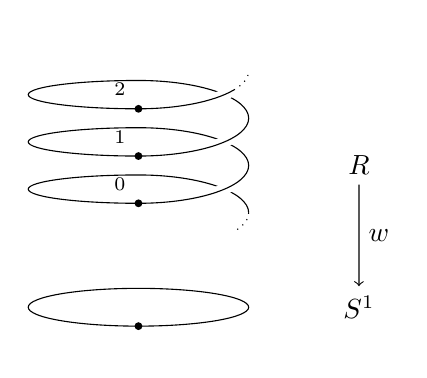
\begin{tikzpicture}[xscale=1.4,yscale=.6]
    \node (R) at (2,1) {$\mathbb{R}$};
    \node (S1) at (2,-2) {$S^1$};
    \draw[->] (R) -- node[auto] {$w$} (S1);
    \draw (0,-2) ellipse (1 and .4);
    \draw[dotted] (1,0) arc (0:-30:1 and .8);
    \draw (1,0) arc (0:90:1 and .8) arc (90:270:1 and .3) coordinate (t1);
    \draw[white,line width=4pt] (t1) arc (-90:90:1 and .8);
    \draw (t1) arc (-90:90:1 and .8) arc (90:270:1 and .3) coordinate (t2);
    \draw[white,line width=4pt] (t2) arc (-90:90:1 and .8);
    \draw (t2) arc (-90:90:1 and .8) arc (90:270:1 and .3) coordinate (t3);
    \draw[white,line width=4pt] (t3) arc (-90:90:1 and .8);
    \draw (t3) arc (-90:-30:1 and .8) coordinate (t4);
    \draw[dotted] (t4) arc (-30:0:1 and .8);
    \node[fill,circle,inner sep=1pt,label={below:\scriptsize \base}] at (0,-2.4) {};
    \node[fill,circle,inner sep=1pt,label={above left:\scriptsize 0}] at (0,.2) {};
    \node[fill,circle,inner sep=1pt,label={above left:\scriptsize 1}] at (0,1.2) {};
    \node[fill,circle,inner sep=1pt,label={above left:\scriptsize 2}] at (0,2.2) {};
  \end{tikzpicture}
  \caption{The winding map in classical topology}\label{fig:winding}
\end{figure}

Now in classical homotopy theory, where $\Sn^1$ is regarded as a topological space, we may proceed as follows.
Consider the ``winding'' map $w:\mathbb{R}\to \Sn ^1$, which looks like a helix projecting down onto the circle (see \autoref{fig:winding}).
This map $w$ sends each point on the helix to the point on the circle that it is ``sitting above''.
It is a fibration, and the fiber over each point is isomorphic to the integers.
If we lift the path that goes counterclockwise around the loop on the bottom, we go up one level in the helix, incrementing the integer in the fiber.
Similarly, going clockwise around the loop on the bottom corresponds to going down one level in the helix, decrementing this count.
This fibration is called the \emph{universal cover} of the circle.

Now a basic fact in classical homotopy theory is that a map $E_1\to E_2$ of fibrations over $B$ which is a homotopy equivalence between $E_1$ and $E_2$ induces a homotopy equivalence on all fibers.
(We have already seen the type-theoretic version of this as well in \autoref{thm:total-fiber-equiv}.)
Since $\mathbb{R}$ and $P_{\base} S^1$ are both contractible topological spaces, they are homotopy equivalent, and thus their fibers $\Z$ and $\Omega(\Sn ^1)$ over the basepoint are also homotopy equivalent.

\subsection{The universal cover in type theory}
\label{sec:pi1s1-universal-cover}

Let us consider how we might express the preceeding proof in type theory.
We have already remarked that the path fibration of $\Sn^1$ is represented by the type family $(x\mapsto (\base=x))$.
We have also already seen a good candidate for the universal cover of $\Sn^1$: it's none other than the type family $c:\Sn^1\to\type$ which we defined in \autoref{sec:pi1s1-initial-thoughts}!
By definition, the fiber of this family over $\base$ is $\Z$, while the effect of transporting around $\lloop$ is to add one --- thus it behaves just as we would expect from \autoref{fig:winding}.

However, since we don't know yet that this family behaves like a universal cover is supposed to (for instance, that its total space is contractible), we use a different name for it.
For reference, therefore, we repeat the definition.

\begin{defn}[Universal Cover of $\Sn^1$] \label{S1-universal-cover}
  Define $\code : \Sn ^1 \to \type$ by circle-recursion, with 
  \begin{align*}
    \code(\base) &\defeq \Z \\
    \apfunc{\code}({\lloop}) &\defid \ua(\Zsuc).
  \end{align*}
\end{defn}

We emphasize briefly the definition of this family, since it is so different from how one usually defines covering spaces in classical homotopy theory.
To define a function by circle recursion, we need to find a point and a
loop in the target.  In this case, the target is $\type$, and the point
we choose is $\Z$, corresponding to our expectation that the
fiber of the universal cover should be the integers.  The loop we choose
is the successor/predecessor isomorphism on $\Z$, which
corresponds to the fact that going around the loop in the base goes up
one level on the helix.  Univalence is necessary for this part of the
proof, because we need to convert \emph{non-trivial} equivalence on $\Z$ into an identity.  

We call this the fibration of ``codes'', because its elements are combinatorial data that act as codes for paths on the circle: the integer $n$ codes for the path which loops around the circle $n$ times.

From this definition, it is simple to calculate that transporting with
$\code$ takes $\lloop$ to the successor function, and 
$\opp{\lloop}$ to the predecessor function:
\begin{lem} \label{lem:transport-s1-code}
\id{\transfib \code \lloop x} {x + 1} and 
\id{\transfib \code {\opp \lloop} x} {x - 1}
\end{lem}
\begin{proof}
For the first, we calculate as follows:
\begin{alignat*}{2}
{\transfib \code \lloop x} 
&= \transfib {A \mapsto A} {(\ap{\code}{\lloop})} x &&\quad\text{by associativity}\\
&= \transfib {A \mapsto A} {\ua (\Zsuc)} x &&\quad\text{by computation for $\rec{\Sn^1}$}\\
&= x + 1 &&\quad\text{computation for \ua}
\end{alignat*}
The second follows from the first, because $\transfib B p-$  and ${\transfib B {\opp p}{-}}$ are always inverses, so ${\transfib\code {\opp \lloop}{-}}$ must be the inverse of $\Zsuc$.
\end{proof}

We can now see what was wrong with our first approach: we defined $f$ and $g$ only on the fibers $\Omega(\Sn^1)$ and \Z, when we should have defined a whole morphism \emph{of fibrations} over $\Sn^1$.
In type theory, this means we should have defined functions having types
\begin{align}
  \prd{x:\Sn^1} &((\base=x) \to \code(x)) \qquad\text{and/or} \label{eq:pi1s1-encode}\\
  \prd{x:\Sn^1} &(\code(x) \to (\base=x))\label{eq:pi1s1-decode}
\end{align}
instead of only the special cases of these when $x$ is \base.
This is also an instance of a common observation in type theory: when attempting to prove something about particular inhabitants of some inductive type, it is often easier to generalize the statement so that it refers to \emph{all} inhabitants of that type, which we can then prove by induction.
Looked at in this way, the proof of $\Omega(\Sn^1)=\Z$ fits into the same pattern as the characterization of the identity types of coproducts and natural numbers in \autoref{sec:compute-coprod,sec:compute-nat}.

At this point, there are two ways to finish the proof.
We can continue mimicking the classical argument by constructing~\eqref{eq:pi1s1-encode} or~\eqref{eq:pi1s1-decode} (it doesn't matter which), proving that a homotopy equivalence between total spaces induces an equivalence on fibers, and then that the total space of the universal cover is contractible.
The first type-theoretic proof of $\Omega(\Sn^1)=\Z$ followed this pattern; we call it the \emph{homotopy-theoretic} proof.

Later, however, we discovered that there is an alternative proof, which has a more type-theoretic feel and more closely follows the proofs in \autoref{sec:compute-coprod,sec:compute-nat}.
In this proof, we directly construct both~\eqref{eq:pi1s1-encode} and~\eqref{eq:pi1s1-decode}, and prove that they are mutually inverse by calculation.
We will call this the \emph{type-theoretic} or \emph{encode/decode} proof, because we call the functions~\eqref{eq:pi1s1-encode} and~\eqref{eq:pi1s1-decode} \emph{encode} and \emph{decode} respectively.
Both proofs use the same construction of the cover given above.
Where the classical proof induces an equivalence on fibers from an equivalence between total spaces, the encode/decode proof constructs the inverse map (\emph{decode}) explicitly as a map between fibers.
And where the classical proof uses contractibility, the type-theoretic proof uses path induction, circle induction, and integer induction.
These are the same tools used to prove contractibility---indeed, path induction \emph{is} essentially contractibility of the path fibration composed with $\mathsf{transport}$---but they are applied in a different way.

Since this is a book about homotopy type theory, we present the type-theoretic proof first.
A homotopy theorist who gets lost is encouraged to skip to the homotopy-theoretic proof (\autoref{subsec:pi1s1-homotopy-theory}).

\subsection{The type-theoretic proof}
\label{subsec:pi1s1-encode-decode}

We begin with the function~\eqref{eq:pi1s1-encode} that maps paths to codes:
\begin{defn}
Define $\encode : \prd{x : \Sn ^1} \rightarrow (\base=x) \rightarrow  \code(x)$ by 
\[
\encode \: p \defeq \transfib{\code} p 0
\]
(we leave the argument $x$ implicit).  
\end{defn}
Encode is defined by lifting a path into the universal cover, which
determines an equivalence, and then applying the resulting equivalence
to $0$.  
The interesting thing about this function is that it computes a concrete
number from a loop on the circle, when this loop is represented using
the abstract groupoidal framework of HoTT.  To gain an
intuition for how it does this, observe that by the above lemmas,
$\transfib \code \lloop x$ is the successor function $\Zsuc$ and $\transfib \code {\opp
  \lloop} x$ is the predecessor function $\Zpred$.
Further, $\mathsf{transport}$ is functorial (\autoref{cha:basics}), so
\[\transfib{\code} {\lloop \ct \lloop}{-}
\quad\text{is}\quad
(\transfib \code \lloop-) \circ (\transfib \code \lloop-)\]
and so on.
Thus, when $p$ is a composition like 
\[
\lloop \ct \opp \lloop \ct \lloop \ct ...
\]
$\transfib{\code}{p}{-}$ will compute a composition of functions like
\[
\Zsuc \circ \Zpred \circ \Zsuc \circ ... 
\]
Applying this composition of functions to 0 will compute the
\emph{winding number} of the path---how many times it goes around the
circle, with orientation marked by whether it is positive or negative,
after inverses have been canceled.  Thus, the computational behavior of
$\encode$ follows from the reduction rules for higher-inductive types and
univalence, and the action of $\mathsf{transport}$ on compositions and inverses.

Note that the instance $\encode' \defeq \encode_{\base}$ has type 
$(\id \base \base) \rightarrow \Z$.
This will be one half of our desired equivalence; indeed, it is exactly the function $g$ defined in \autoref{sec:pi1s1-initial-thoughts}.

Similarly, the function~\eqref{eq:pi1s1-decode} is a generalization of the function $\lloop^-$ from \autoref{sec:pi1s1-initial-thoughts}.

\begin{defn}\label{thm:pi1s1-decode}
Define $\decode : \prd{x : \Sn ^1}\code(x) \rightarrow (\base=x)$ by 
circle induction on $x$.  It suffices to give a function 
${\code(\base) \rightarrow (\base=\base)}$, for which we use $\lloop^-$, and 
to show that $\lloop^-$ respects the loop.  
\end{defn}

\begin{proof}
To show that $\lloop^-$ respects the loop, it suffices to give a path
from $\lloop^-$ to itself that lies over $\lloop$. 
Formally, this means a path from $\transfib {(x' \mapsto \code(x')
\rightarrow (\base=x'))} {\lloop} {\lloop^-}$ to $\lloop^-$.  We define such a
path as follows:
\begin{align*}
  \MoveEqLeft \transfib {(x' \mapsto \code(x') \rightarrow (\base=x'))} \lloop {\lloop^-}\\
&= \transfibf {x'\mapsto (\base=x')}(\lloop) \circ {\lloop^-} \circ \transfibf \code ({\opp \lloop}) \\
&= (- \ct \lloop) \circ (\lloop^-) \circ \transfibf \code ({\opp \lloop}) \\
&= (- \ct \lloop) \circ (\lloop^-) \circ \Zpred \\
&= (n \mapsto \lloop^{n - 1} \ct \lloop)                 
\end{align*}
On the first line, we apply the characterization of $\mathsf{transport}$
when the outer connective of the fibration is $\rightarrow$, which
reduces the $\mathsf{transport}$ to pre- and post-composition with
$\mathsf{transport}$ at the domain and range types.  On the second line,
we apply the characterization of $\mathsf{transport}$ when the type family
is $x\mapsto \id{\base}{x}$, which is post-composition of paths.  On the third line,
we use the action of $\code$ on $\opp \lloop$ from
\autoref{lem:transport-s1-code}.  And on the fourth line, we simply
reduce the function composition.  Thus, it suffices to show that for all
$n$, \id{\lloop^{n - 1} \ct \lloop}{\lloop^{n}}, which is an easy
induction, using the groupoid laws.  
\end{proof}

We can now show that $\encode$ and $\decode$ are quasi-inverses.
What used to be the difficult direction is now easy!

\begin{lem} \label{lem:s1-decode-encode}  For all 
for all $x: \Sn ^1$ and $p : \id \base x$, $\id
{\decode_x({{\encode_x(p)}})} p$.  
\end{lem}

\begin{proof}
By path induction, it suffices to show that 
$\id {\decode_{\base}({{\encode_{\base}(\refl{\base})}})} {\refl{\base}}$.
But
${\encode_{\base}(\refl{\base})} \jdeq 
 \transfib{\code}{\refl{\base}} 0 \jdeq 0$, and $\decode_{\base}(0)
 \jdeq \lloop^ 0 \jdeq \refl{\base}$.  
\end{proof}

The other direction is not much harder.

\begin{lem} \label{lem:s1-encode-decode} For all 
$x: \Sn ^1$ and $c : \code(x)$, we have $\id
{\encode_x({{\decode_x(c)}})} c$.  
\end{lem}

\begin{proof}
The proof is by circle induction.  It suffices to show the case for
\base, because the case for \lloop is a path between paths in
$\Z$, which is immediate because $\Z$ is a set.  

Thus, it suffices to show, for all $n : \Z$, that
\[
\id {\encode'(\lloop^n)} {n}
\]
The proof is by induction, using \cref{thm:looptothe}.  

\begin{itemize}

\item In the case for $0$, the result is true by definition.

%% \item In the case for $1$, ${\encode'(\lloop^1)}$ reduces to 
%% $\transfib{\code}{\lloop}{0}$, which by
%% \autoref{lem:transport-s1-code} is $0 + 1 = 1$.  

\item In the case for $n+1$, 
\begin{alignat*}{2}
 {\encode'(\lloop^{n+1})}
&= {\encode'(\lloop^{n} \ct \lloop)} &&\quad\text{by definition of $\lloop^{-}$} \\
&= \transfib{\code}{(\lloop^{n} \ct \lloop)}{0} &&\quad\text{by definition of $\encode$}\\
&= \transfib{\code}{\lloop}{(\transfib{\code}{\lloop^n}{0})} &&\quad\text{by functoriality}\\
&= {(\transfib{\code}{\lloop^n}{0})} + 1 &&\quad\text{by \autoref{lem:transport-s1-code}}\\
&= n + 1 &&\quad\text{by the IH} \\
\end{alignat*}

\item The case for negatives is analogous.  \qedhere
\end{itemize}
\end{proof}

Finally, we conclude the theorem.

\begin{thm} 
There is a family of equivalences $\prd{x : \Sn ^1} (\eqv {(\base=x)} {\code(x)})$.
\end{thm}
\begin{proof}
The maps $\encode$ and $\decode$ are quasi-inverses by
\autoref{lem:s1-decode-encode,lem:s1-decode-encode}.
\end{proof}

Instantiating at {\base} gives
\begin{cor}\label{cor:omega-s1}
$\eqv {\Omega(\Sn^1,\base)} {\Z}$.
\end{cor}

A simple induction shows that this equivalence takes addition to
composition, so that $\Omega(\Sn ^1) = \Z$ as groups.

\begin{cor} \label{cor:pi1s1}
$\id{\pi_1(\Sn ^1)} {\Z}$, while $\id{\pi_n(\Sn ^1)}0$ for $n>1$.
\end{cor}
\begin{proof}
For $n=1$, we sketched the proof from \autoref{cor:omega-s1} above.
For $n > 1$, we have $\trunc 0 {\Omega^{n}(\Sn ^1)} = \trunc 0 {\Omega^{n-1}(\Omega{\Sn ^1})} = \trunc 0 {\Omega^{n-1}(\Z)}$.
And since $\Z$ is a set, $\Omega^{n-1}(\Z)$ is contractible, so this is trivial.
\end{proof}


\subsection{The homotopy-theoretic proof}
\label{subsec:pi1s1-homotopy-theory}

In \autoref{sec:pi1s1-universal-cover}, we defined the putative universal cover $\code:\Sn^1\to\type$ in type theory, and in \autoref{subsec:pi1s1-homotopy-theory} we defined a map $\encode : \prd{x:\Sn^1} (\base=x) \to \code(x)$ from the path fibration to the universal cover.
What remains for the classical proof is to show that this map induces an equivalence on total spaces because both are contractible, and to deduce from this that it must be an equivalence on each fiber.

We have already seen in \autoref{thm:contr-paths} that the total space $\sm{x:\Sn^1} (\base=x)$ is contractible.
For the other, we have:

\begin{lem}
  The type $\sm{x:\Sn^1}\code(x)$ is contractible.
\end{lem}
\begin{proof}
  We apply the flattening lemma (\autoref{thm:flattening}) with the following values:
  \begin{itemize}
  \item $A\defeq\unit$ and $B\defeq\unit$, with $f$ and $g$ the obvious functions.
    Thus, the base higher inductive type $W$ in the flattening lemma is equivalent to $\Sn^1$.
  \item $C:A\to\type$ is constant at \Z.
  \item $D:\prd{b:B} (\eqv{\Z}{\Z})$ is constant at $\Zsuc$.
  \end{itemize}
  Then the type family $P:\Sn^1\to\type$ defined in the flattening lemma is equivalent to $\code:\Sn^1\to\type$.
  Thus, the flattening lemma tells us that $\sm{x:\Sn^1}\code(x)$ is equivalent to higher inductive type with the following generators, which we denote $R$:
  \begin{itemize}
  \item A function $\mathsf{c}: \Z \to R$.
  \item For each $z:\Z$, a path $\mathsf{p}_z:\mathsf{c}(z) = \mathsf{c}(\Zsuc(z))$.
  \end{itemize}
  We might call this type the \emph{homotopical reals}; it plays the same role as the topological space $\mathbb{R}$ in the classical proof.

  Thus, it remains to show that $R$ is contractible.
  As center of contraction we choose $\mathsf{c}(0)$; we must now show that $x=\mathsf{c}(0)$ for all $x:R$.
  We do this by induction on $R$.
  Firstly, when $x$ is $\mathsf{c}(z)$, we must give a path $q_z:\mathsf{c}(0) = \mathsf{c}(z)$, which we can do by induction on $z:\Z$:
  \begin{alignat*}{2}
    q_0 &\defeq \refl{\mathsf{c}(0)}\\
    q_{n+1} &\defeq q_n \ct \mathsf{p}_n && \quad n\ge 0\\
    q_{n-1} &\defeq q_n \ct \opp{\mathsf{p}_{n-1}} && \quad n\le 0.
  \end{alignat*}
  Secondly, we must show that for any $z:\Z$, the path $q_z$ is transported along $\mathsf{p}_z$ to $q_{z+1}$.
  By transport of paths, this means we want $q_z \ct \mathsf{p}_z = q_{z+1}$.
  This is easy by induction on $z$, using the definition of $q_z$.
  This completes the proof that $R$ is contractible, and thus so is $\sm{x:\Sn^1}\code(x)$.
\end{proof}

\begin{cor}\label{thm:encode-total-equiv}
  The map induced by \encode:
  \[ \tsm{x:\Sn^1} (\base=x) \to \tsm{x:\Sn^1}\code(x) \]
  is an equivalence.
\end{cor}
\begin{proof}
  Both types are contractible.
\end{proof}

\begin{thm}
  $\eqv {\Omega(\Sn^1,\base)} {\Z}$.
\end{thm}
\begin{proof}
  Apply \autoref{thm:total-fiber-equiv} to $\encode$, using \autoref{thm:encode-total-equiv}.
\end{proof}

In essence, the two proofs are not very different: the type-theoretic one may be seen as a ``reduction'' or ``unpackaging'' of the homotopy-theoretic one.
Each has its advantages; the interplay between the two points of view is part of the interest of the subject.

\subsection{The universal cover as an identity system}
\label{sec:pi1s1-idsys}

Note that the fibration $\code:\Sn^1\to\type$ together with $0:\code(\base)$ is a \emph{pointed predicate} in the sense of \autoref{defn:identity-systems}.
From this point of view, we can see that the type-theoretic proof in \autoref{subsec:pi1s1-encode-decode} consists of proving that \code satisfies \autoref{thm:identity-systems}\ref{item:identity-systems3}, while the homotopy-theoretic proof in \autoref{subsec:pi1s1-homotopy-theory} consists of proving that it satisfies \autoref{thm:identity-systems}\ref{item:identity-systems4}.
This suggests a third approach.

\begin{thm}
  The pair $(\code,0)$ is an identity system at $\base:\Sn^1$ in the sense of \autoref{defn:identity-systems}.
\end{thm}
\begin{proof}
  Let $D:\prd{x:\Sn^1} \code(x) \to \type$ and $d:D(\base,0)$ be given; we want to define a function $f:\prd{x:\Sn^1}{c:\code(x)} D(x,c)$.
  By circle induction, it suffices to specify $f(\base):\prd{c:\code(\base)} D(\base,c)$ and verify that $\trans{\lloop}{f(\base)} = f(\base)$.

  Of course, $\code(\base)\jdeq \Z$.
  By \autoref{lem:transport-s1-code} and induction on $n$, we may obtain a path $p_n : \transfib{\code}{\lloop^n}{0} = n$ for any integer $n$.
  Therefore, by paths in $\Sigma$-types, we have a path $\pairpath(\lloop^n,p_n) : (\base,0) = (\base,n)$ in $\sm{x:\Sn^1} \code(x)$.
  Transporting $d$ along this path in the fibration $\hat{D}:(\sm{x:\Sn^1} \code(x)) \to\type$ associated to $D$, we obtain an element of $D(\base,n)$ for any $n:\Z$.
  We define this element to be $f(\base)(n)$:
  \[ f(\base)(n) \defeq \transfib{\hat{D}}{\pairpath(\lloop^n,p_n)}{d}. \]

  Now we need $\transfib{\lam{x} \prd{c:\code(x)} D(x,c)}{\lloop}{f(\base)} = f(\base)$.
  By \autoref{thm:dpath-forall}, this means we need to show that for any $n:\Z$,
  \[ \transfib{\hat D}{\pairpath(\lloop,\refl{\trans\lloop n})}{f(\base)(n)} =_{D(\base,\trans\lloop n)} f(\base)(\trans\lloop n). \]
  Now we have a path $q:\trans\lloop n = n+1$, so transporting along this, it suffices to show
  \begin{multline*}
    \transfib{D(\base)}{q}{\transfib{\hat D}{\pairpath(\lloop,\refl{\trans\lloop n})}{f(\base)(n)}}\\
    =_{D(\base,n+1)} \transfib{D(\base)}{q}{f(\base)(\trans\lloop n)}.
  \end{multline*}
  By a couple of lemmas about transport and dependent application, this is equivalent to
  \[ \transfib{\hat D}{\pairpath(\lloop,q)}{f(\base)(n)} =_{D(\base,n+1)} f(\base)(n+1). \]
  However, expanding out the definition of $f(\base)$, we have
  \begin{align*}
    \transfib{\hat D}{\pairpath(\lloop,q)}{f(\base)(n)}
    &= \transfib{\hat D}{\pairpath(\lloop,q)}{\transfib{\hat{D}}{\pairpath(\lloop^n,p_n)}{d}}\\
    &= \transfib{\hat D}{\pairpath(\lloop^n,p_n) \ct \pairpath(\lloop,q)}{d}\\
    &= \transfib{\hat D}{\pairpath(\lloop^{n+1},p_{n+1})}{d}\\
    &= f(\base)(n+1).
  \end{align*}
  We have used the functoriality of transport, the characterization of composition in $\Sigma$-types (which was an exercise for the reader), and a lemma relating $p_n$ and $q$ to $p_{n+1}$ which we leave it to the reader to state and prove.
  
  This completes the construction of $f:\prd{x:\Sn^1}{c:\code(x)} D(x,c)$.
  Since
  \[f(\base,0) \jdeq \trans{\pairpath(\lloop^0,p_0)}{d} = \trans{\refl{\base}}{d} = d,\]
  we have shown that $(\code,0)$ is an identity system.
\end{proof}

\begin{cor}
  For any $x:\Sn^1$, we have $\eqv{(\base=x)}{\code(x)}$.
\end{cor}
\begin{proof}
  By \autoref{thm:identity-systems}.
\end{proof}

Of course, this proof also contains essentially the same elements as the previous two.
Roughly, we can say that it unifies the proofs of \autoref{thm:pi1s1-decode,lem:s1-encode-decode}, performing the requisite inductive argument only once in a generic case.


\section{Connectedness of suspensions}
\label{sec:conn-susp}

\begin{defn}
  A type $A$ is called \emph{$n$-connected} if $\trunc nA$ is contractible.
\end{defn}

\begin{lem}
  \label{connectedtotruncated}
  Let $n\ge-2$, $A:\type$ and $B:\typele{n}$ and assume moreover that $A$ is
  $n$-connected.

  Then every map from $A$ to $B$ is constant in the sense that the constant map
  operation
  \[\function{B}{(A\to{}B)}{b}{\lamu{x:A} b}\]
  is an equivalence.
\end{lem}
\begin{proof}
  This is just an application of the universal property. Note that
  \[(\trunc nA\to{}B)=(\unit\to{}B)=B \qedhere\]
\end{proof}

The aim of this section is to prove that the operation of suspension increases
connectedness.

\begin{thm} \label{thm:suspension-increases-connectedness}
  Let $n\ge-2$ and $A:\type$.

  If $A$ is $n$-connected then the suspension of $A$ is $(n+1)$-connected.
\end{thm}

\begin{proof}
  By definition, the suspension of $A$ is $\unit\sqcup^A\unit$, so we need to
  prove that the following type is contractible:

  \[\trunc{n+1}{\unit\sqcup^A\unit}\]

  By \autoref{reflectcommutespushout} we know that
  $\trunc{n+1}{\unit\sqcup^A\unit}$ is a pushout in $\typelep{n+1}$ of the diagram
  \[\xymatrix{\trunc{n+1}A \ar[d] \ar[r] & \trunc{n+1}{\unit} \\
    \trunc{n+1}{\unit} & }\]

  Given that $\trunc{n+1}{\unit}=\unit$, the type
  $\trunc{n+1}{\unit\sqcup^A\unit}$ is also a pushout of the following diagram in
  $\typelep{n+1}$ (because both diagrams are equal)
  \[\Ddiag=\xymatrix{\trunc{n+1}A \ar[d] \ar[r] & \unit \\
    \unit & }\]

  We will now prove that $\unit$ is also a pushout of $\Ddiag$ in
  $\typelep{n+1}$.

  \bigskip

  Let $E$ be an $(n+1)$-truncated type; we need to prove that the following map
  is an equivalence
  \[\function{(\unit\to{}E)}{\cocone{\Ddiag}{E}}{y}
  {(y,y,\lamu{u:{\trunc{n+1}A}} \refl{y(\ttt)})}\]
  where we recall that $\cocone{\Ddiag}{E}$ is the type
  \[\sm{f:\unit\to{}E}{g:\unit\to{}E}(\trunc{n+1}A\to
  (f(\ttt)=_E{}g(\ttt)))\]

  The map $\function{(\unit\to{}E)}{E}{f}{f(\ttt)}$ is an equivalence, hence
  we also have
  \[\cocone{\Ddiag}{E}=\sum_{x:E}\sum_{y:E}(\trunc{n+1}A\to(x=_Ey))\]

  Now $A$ is $n$-connected hence so is $\trunc{n+1}A$ because
  $\trunc n{\trunc{n+1}A}=\trunc nA=\unit$, and $(x=_Ey)$ is $n$-truncated because
  $E$ is $(n+1)$-connected. Hence by \autoref{connectedtotruncated} the
  following map is an equivalence
  \[\function{(x=_Ey)}{(\trunc{n+1}A\to(x=_Ey))}{p}{\lam{z} p}\]

  Hence we have
  \[\cocone{\Ddiag}{E}=\sm{x:E}{y:E}(x=_Ey)\]

  But the following map is an equivalence
  \[\function{E}{\sm{x:E}{y:E}(x=_Ey)}{x}{(x,x,\refl{x})}\]

  Hence
  \[\cocone{\Ddiag}{E}=E\]

  Finally we get an equivalence
  \[(\unit\to{}E)\simeq\cocone{\Ddiag}{E}\]

  We can now unfold the definitions in order to get the explicit expression of
  this map, and we see easily that this is exactly the map we had at the
  beginning.

  \bigskip

  Hence we proved that $\unit$ in a pushout of $\Ddiag$ in $\typelep{n+1}$. Using
  uniqueness of pushouts we get that $\trunc{n+1}{\unit\sqcup^A\unit}=\unit$
  which proves that the suspension of $A$ is $(n+1)$-connected.
\end{proof}

\begin{cor} \label{cor:sn-connected}
  For all $n:\N$, the sphere $\Sn^n$ is $(n-1)$-connected.
\end{cor}

\begin{proof}
  We prove this by induction on $n$.

  For $n=0$ we have to prove that $\Sn^0$ is inhabited which is clear.

  Let $n:\N$ such that $\Sn^n$ is $(n-1)$-connected. By definition $\Sn^{n+1}$
  is the suspension of $\Sn^n$ hence by the previous lemma $\Sn^{n+1}$ is
  $n$-connected.
\end{proof}

\section{\texorpdfstring{$\pi_{k \le n}$}{π\_(k≤n)} of an \texorpdfstring{$n$}{n}-connected space and \texorpdfstring{$\pi_{k < n}(\Sn ^n)$}{π\_(k<n)(Sⁿ)}}
\label{sec:pik-le-n}

Let $(A,a)$ be a pointed type and $n:\N$.  Recall from
\autoref{thm:homotopy-groups} that if $n>0$ the set $\pi_n(A,a)$ has a group
structure, and if $n>1$ the group is Abelian.

We can now say something about homotopy groups of $n$-truncated and
$n$-connected types.

\begin{lem}
  If $A$ is $n$-truncated and $a:A$, then we have
  \[\forall k>n,\ \pi_k(A,a)=\unit\]
\end{lem}

\begin{proof}
  Indeed, taking the loop space of an $n$-truncated type gives an
  $(n-1)$-truncated type, hence $\Omega^k(A,a)$ is $(n-k)$-truncated and we have
  $(n-k)\le-1$ so $\Omega^k(A,a)$ is \anhprop. But $\Omega^k(A,a)$ is inhabited,
  so it is actually contractible and
  $\pi_k(A,a)=\trunc0{\Omega^k(A,a)}=\trunc0{\unit}=\unit$.
\end{proof}

\begin{lem} \label{lem:pik-nconnected}
  If $A$ is $n$-connected and $a:A$, then we have
  \[\forall k\le{}n,\ \pi_k(A,a)=\unit\]
\end{lem}

\begin{proof}
  We have the following sequence of equalities:

  \begin{align*}
    \pi_k(A,a) &= \trunc0{\Omega^k(A,a)} \\
    &= \Omega^k(\trunc k{(A,a)}) \\
    &= \Omega^k(\trunc k{\trunc n{(A,a)}}) \\
    &= \Omega^k(\trunc k{\unit}) \\
    &= \Omega^k(\unit) \\
    &= \unit
  \end{align*}

  The third line uses the fact that $k\le{}n$ in order to use that
  $\truncf k\circ\truncf n=\truncf k$ and the fourth line uses the fact that $A$ is
  $n$-connected.
\end{proof}

\begin{cor}[$\pi_{k<n}(\Sn ^n)$]
For all $n$ and $k$, if $k < n$, then $\pi_k(\Sn ^n) = \unit$.  
\end{cor}
\begin{proof}
$\Sn$ is $n\mathord{-}1$-connected by \autoref{cor:sn-connected}.  Therefore
\autoref{lem:pik-nconnected} gives the result.  
\end{proof}

\section{Fiber sequences and the long exact sequence of homotopy groups}
\label{sec:long-exact-sequence-homotopy-groups}
Given a fibration $E\twoheadrightarrow B$ with fiber $F$, there is a relation
between the homotopy groups of $F$, $E$ and $B$ in the form of a long exact
sequence. We will start by defining the fiber sequence associated to a map
between pointed spaces

\begin{defn}
  A \define{pointed space} is a space $X$ together with a point $x_0:X$.

  A \define{pointed map} between two pointed spaces $(X,x_0)$ and $(Y,y_0)$ is a
  map $f$ between $X$ and $Y$ together with a path $f_0:f(x_0)=y_0$.
\end{defn}

\begin{defn}
  Given a pointed space $X$, the \define{loop space} of $X$ is the type
  $(x_0=x_0)$ (where $x_0$ is the base point of $X$).
\end{defn}

\begin{defn}
  Given a map between pointed spaces $f:X\to{}Y$, we define a function $\Omega
  f:\Omega X \to \Omega Y$ by
  \[(\Omega f)(p) \defeq \rev{f_0}\ct\ap{f}{p}\ct f_0\]
\end{defn}


\begin{defn}
  A \define{fiber sequence} is a (possibly bounded) sequence of pointed types
  and pointed maps:
  \[\xymatrix{\dots \ar[r] & X_{n+1} \ar[r] & X_n \ar[r] & X_{n-1} \ar[r] &
    \dots}\]
  %
  such that for every $n$ the map $X_{n+1}\to{}X_n$ is the fiber of the map
  $X_n\to{}X_{n-1}$.
\end{defn}

Given a map $f:X\to Y$ it is easy to extend it to a fiber sequence infinite to
the left and ending by $f$ by taking the iterated fiber. The following lemma
shows that what we obtain is the sequence of iterated loop spaces (at the base
point) of the base space, the total space and the fiber.

\begin{lem}
  Let $f:X\to Y$ be a map of pointed spaces. Then the fiber of the fiber of $f$
  is equivalent to $\Omega Y$, and the map from the fiber iterated three times
  of $f$ (which is $\Omega X$) to the fiber of the fiber of $f$ (which is
  $\Omega Y$) is $\Omega f\circ\rev{-}$.
\end{lem}
\begin{proof}
  The fiber of the fiber of $f$ is
  \begin{align*}
    \setof{z:\hfib{f}{y_0} | \proj{1}(z) = x_0} &=
    \setof{x:A,p:f(x)=y_0 | x = x_0}
  \end{align*}
  %
  So a point of this space $F$ is a triple consisting of a point $x:X$, a path
  $p$ from $f(x)$ to $y_0$ and a path $q$ from $x$ to $x_0$. Let’s prove that
  $F$ and $\Omega Y$ are equivalent.

  We define the following two maps
  %
  \begin{align*}
    g &: F \to \Omega Y\\
    g(x,p,q) &= \rev{p}\ct\ap{f}{q}\ct f_0
  \end{align*}
  %
  \begin{align*}
    h &: \Omega Y \to F\\
    h(p) &= (x_0, f_0\ct\rev{p}, \refl{x_0})
  \end{align*}
  %
  We can now check that they are inverse to each other:
  %
  \begin{align*}
    g(h(p)) &= g(x_0, f_0\ct\rev{p}, \refl{x_0}) \\
    &= \rev{(f_0\ct\rev{p})}\ct\ap{f}{\refl{x_0}}\ct f_0 \\
    &= \rev{(\rev{p})}\ct\rev{f_0}\ct f_0 \\
    &= p\\
    &\\
    h(g(x,p,q)) &= h(\rev{p}\ct\ap{f}{q}\ct f_0)\\
    &= (x_0, f_0\ct\rev{(\rev{p}\ct\ap{f}{q}\ct f_0)}, \refl{x_0}) \\
    &= (x_0, f_0\ct\rev{f_0}\ct\rev{\ap{f}{q}}\ct\rev{(\rev{p})}, \refl{x_0}) \\
    &= (x_0, \rev{\ap{f}{q}}\ct p, \refl{x_0}) \\
  \end{align*}
  %
  But we have $(x,p,q)=(x_0, \rev{\ap{f}{q}}\ct p, \refl{x_0})$ because $q$ is
  an equality between $x$ and $x_0$, the paths $p$ and $\rev{\ap{f}{q}}\ct p$
  are equal over $q$, and the paths $q$ and $\refl{x_0}$ are equal over $q$.

  We have the following fiber sequence
  %
  \[\xymatrix{F' \ar^-k[r] & F \ar[r] & F_0 \ar[r] & X \ar[r] & Y}\]
  %
  and we’ve constructed equivalences $e_X:\eqv{\Omega X}{F'}$ and
  $e_Y\eqv{\Omega Y}{F}$. The map $\Omega X\to\Omega Y$ obtained in this way
  sends a loop $p$ to the following path:
  %
  \begin{align*}
    e_Y^{-1}(k(e_X(p))) &=
    e_Y^{-1}(k((x_0,f_0),\refl{x_0}\ct\rev{p},\refl{(x_0,f_0)}) \\
    &= e_Y^{-1}((x_0,f_0),\refl{x_0}\ct\rev{p}) \\
    &= \rev{f_0}\ct\ap{f}{\refl{x_0}\ct\rev{p}}\ct f_0 \\
    &= (\Omega f)(\rev{p})
  \end{align*}
\end{proof}

From this fiber sequence we will deduce an exact sequence of pointed sets.

\begin{defn}
  An \define{exact sequence} is a (possibly bounded) sequence of pointed sets
  and pointed maps:
  \[\xymatrix{\dots \ar[r] & X_{n+1} \ar[r] & X_n \ar[r] & X_{n-1} \ar[r] &
    \dots}\]
  %
  such that for every $n$ the image of the map $X_{n+1}\to{}X_n$ (cf
  \autoref{def:modal-image}) is equal to the kernel of the map $X_n\to{}X_{n-1}$
  (the kernel is the set of elements of $X_n$ whose image is equal to the base
  point of $X_{n-1}$).

  If the sets $X_n$ are groups, we require moreover that the maps are morphisms
  of groups.
\end{defn}

\begin{lem}
  The $0$-truncation of a fiber sequence is an exact sequence.
\end{lem}
\begin{proof}
  Given a fiber sequence
  %
  \[\xymatrix{\hfib{f}{z_0} \ar^-g[r] & Y \ar^-f[r] & Z}\]
  %
  we need to prove that
  %
  \[\xymatrix{\trunc{0}{\hfib{f}{z_0}} \ar^-{\trunc0g}[r] & \trunc0{Y}
    \ar^-{\trunc0{f}}[r] & \trunc0{Z}}\]
  %
  is exact.

  We need to prove that $\im(\trunc0g)\subset\ker(\trunc0f)$ and
  $\ker(\trunc0f)\subset\im(\trunc0)$.

  The first inclusion is equivalent to $\trunc0g\circ\trunc0f=0$, which is true
  by functoriality of 0-truncation and using the fact that $g\circ f=0$.

  For the second inclusion assume we have $y':\trunc0Y$ and
  $p':\trunc0f(y')=\tproj0{z_0}$, we want to prove that there merely exists a
  $t:\hfib{f}{z_0}$ such that $g(t)=y'$.

  We want to prove a mere proposition, hence we can assume that $y'$ is of the
  form $\tproj0y$ for some $y:Y$ and then $p'$ is of type
  $\tproj0{f(y)}=\tproj0{z_0}$. According to \autoref{thm:path-truncation} this
  type is equivalent to $\trunc{-1}{f(y)=z_0}$ hence we can assume that $p'$ is
  of the form $\tproj{-1}{p}$ for some $p:f(y)=z_0$. But now the pair $(y,p)$ is
  an element of $\tproj0{\hfib{f}{z_0}}$ whose image by $\trunc0g$ is
  $\tproj0y=y'$ which is what we want.
\end{proof}

\begin{thm}
  Let $f:X\to{}Y$ be a pointed map between pointed spaces with fiber $F$. Then
  we have a long exact sequence of homotopy groups:
  %
  \[
  \xymatrix{
    \vdots & \vdots & \vdots \ar[lld] \\
    \pi_k(F) \ar[r] & \pi_k(X) \ar[r] & \pi_k(Y) \ar[lld] \\
    \vdots & \vdots & \vdots \ar[lld] \\
    \pi_2(F) \ar[r] & \pi_2(X) \ar[r] & \pi_2(Y) \ar[lld] \\
    \pi_1(F) \ar[r] & \pi_1(X) \ar[r] & \pi_1(Y) \ar[lld]\\
    \pi_0(F) \ar[r] & \pi_0(X) \ar[r] & \pi_0(Y)}
  \]
\end{thm}
\begin{proof}
  This is the exact sequence obtained by taking the $0$-truncation of the fiber
  sequence associated to $f$. Note that $\pi_k$ is a group for $k\ge1$ and the
  maps $\pi_k(F)\to\pi_k(X)$ and $\pi_k(X)\to\pi_k(Y)$ are morphisms of groups.

  The fact that the maps $\pi_{k+1}(Y)\to\pi_k(F)$ are also morphisms of groups
  is not immediately obvious but can be easily checked using the formulas above.
\end{proof}

The usual properties of exact sequences of abelian groups can be proved as
usual. In particular we have:
\begin{lem}
  In an exact sequence of abelian groups
  %
  \[\xymatrix{0 \ar[r]& G \ar^f[r] & H \ar[r] & 0}\]
  %
  the map $f$ is an isomorphism of groups.
\end{lem}
\begin{proof}
  The left-hand side of the diagram shows that the kernel of $f$ is $\{0\}$,
  hence $f$ is injective because it’s a group morphism. Moreover the right-hand
  side of the diagrams shows that $f$ is surjective. Hence $f$ is an isomorphism
  of groups by \autoref{thm:mono-surj-equiv}.
\end{proof}

\section{The Hopf fibration}
\label{sec:hopf}

In this section we will define the \emph{Hopf fibration} which was already
mentioned in \autoref{hopf-fibration}:

\begin{thm}[Hopf Fibration]
There is a fibration $H$ over $\Sn ^2$ whose fibers are $\Sn ^1$ and
whose total space is $\Sn ^3$.
\end{thm}

The Hopf fibration will allow us to compute several homotopy groups of
spheres. Indeed, we have the following long exact sequence of homotopy groups
associated to the Hopf fibration (see
\autoref{sec:long-exact-sequence-homotopy-groups}):

\[
\xymatrix{
  \pi_k(\Sn^1) \ar[r] & \pi_k(\Sn^3) \ar[r] & \pi_k(\Sn^2) \ar[lld] \\
  \vdots & \vdots & \vdots \ar[lld] \\
  \pi_2(\Sn^1) \ar[r] & \pi_2(\Sn^3) \ar[r] & \pi_2(\Sn^2) \ar[lld] \\
  \pi_1(\Sn^1) \ar[r] & \pi_1(\Sn^3) \ar[r] & \pi_1(\Sn^2)}
\]

We’ve already computed all $\pi_n(\Sn^1)$ and $\pi_k(\Sn^n)$ for $k<n$, so the
long exact sequence becomes the following:

\[
\xymatrix{
  0 \ar[r] & \pi_k(\Sn^3) \ar[r] & \pi_k(\Sn^2) \ar[lld] \\
  \vdots & \vdots & \vdots \ar[lld] \\
  0 \ar[r] & \pi_3(\Sn^3) \ar[r] & \pi_3(\Sn^2) \ar[lld] \\
  0 \ar[r] & 0 \ar[r] & \pi_2(\Sn^2) \ar[lld] \\
  \Z \ar[r] & 0 \ar[r] & 0}
\]

In particular we get the following result:

\begin{cor} \label{cor:pis2-hopf}
  We have $\eqv{\pi_2(\Sn^2)}{\Z}$ and $\eqv{\pi_k(\Sn^3)}{\pi_k(\Sn^2)}$ for
  every $k\ge3$ (where the map is induced by the Hopf fibration, seen as a map
  from the total space $\Sn^3$ to the base space $\Sn^2$).
\end{cor}

Given that the double loop space of the circle is contractible, we actually get
the slightly more precise result that the Hopf fibration induces an equivalence
$\eqv{\Omega^2(\Sn^3)}{\Omega^2(\Sn^2)}$. In classical homotopy theory this
would be a consequence of Whitehead’s theorem, but Whitehead’s theorem is not
necessarily valid in homotopy type theory. We will not use the more precise
version here though.

We first start with a lemma explaining how to construct fibrations over
pushouts.

\begin{lem}\label{lem:fibration-over-pushout}
  Let $\Ddiag=Y\xleftarrow{j}X\xrightarrow{k}Z$ be a span and assume
  that we have
  \begin{itemize}
  \item Two fibrations $E_Y:Y\to\type$ and $E_Z:Z\to\type$
  \item An equivalence $e_X$ between $E_Y\circ j:X\to\type$ and $E_Z\circ
    k:X\to\type$, ie
    \[e_X:\prd{x:X}\eqv{E_Y(j(x))}{E_Z(k(x))}\]
  \end{itemize}

  Then we can construct a fibration $E:Y\sqcup^XZ\to\type$ such that
  \begin{itemize}
  \item For all $y:Y$, $E(\inl(y))\judgeq E_Y(y)$
  \item For all $z:Z$, $E(\inr(z))\judgeq E_Z(z)$
  \item For all $x:X$, $\map E{\glue(x)}=\ua(e_X(x))$ (note that both sides of
    the equation are paths in $\type$ from $E_Y(j(x))$ to $E_Z(k(x))$)
  \end{itemize}

  Moreover the total space of this fibration fits in the following pushout
  square:

  \[\xymatrix{ \sm{x:X}E_Y(j(x)) \ar[r]_\sim^{\idfunc\times e_X}
    \ar[d]_{j\times\idfunc} &
    \sm{x:X}E_Z(k(x)) \ar[r]^{k\times\idfunc}
    & \sm{z:Z}E_Z(z) \ar[d]^\inr \\
    \sm{y:Y}E_Y(y) \ar[rr]_\inl & & \sm{t:Y\sqcup^XZ}E(t) }\]
\end{lem}

\begin{proof}
  We define $E$ by simple elimination on the pushout $Y\sqcup^XZ$. We need for
  that to specify the value of $E$ on elements of the form $\inl(y)$, $\inr(z)$
  and the action of $E$ on paths $\glue(x)$, so we can just choose the following
  values:
  \begin{align*}
    E(\inl(y)) & \defeq E_Y(y)\\
    E(\inr(z)) & \defeq E_Z(z)\\
    \map E{\glue(x)} & \defid \ua(e_X(x))
  \end{align*}

  To see that the total space of this fibration is a pushout, we apply the
  flattening lemma (\autoref{thm:flattening}) with the following values:
  \begin{itemize}
  \item $A\defeq Y+Z$, $B\defeq X$ and $f,g:B\to A$ are defined by
    $f(x)\defeq\inl(j(x))$, $g(x)\defeq\inr(k(x))$
  \item The type family $C:A\to\type$ is defined by
    \begin{align*}
      C(\inl(y)) & \defeq E_Y(y)\\
      C(\inr(z)) & \defeq E_Z(z)
    \end{align*}
  \item The family of equivalences $D:\prd{b:B}C(f(b))\simeq C(g(b))$ is defined
    to be $e_X$
  \end{itemize}

  The base higher inductive type $W$ in the flattening lemma is equivalent to
  the pushout $Y\sqcup^XZ$ and the type family $P:Y\sqcup^XZ\to\type$ is
  equivalent to the $E$ defined above.

  Thus the flattening lemma tells us that $\sm{t:Y\sqcup^XZ}E(t)$ is equivalent
  the higher inductive type ${E^{\mathrm{tot}}}'$ with the following generators:
  \begin{itemize}
  \item A function $\mathsf{z}:\sm{a:Y+Z}C(a)\to {E^{\mathrm{tot}}}'$
  \item For each $x:X$ and $t:E_Y(j(x))$, a path
    $\mathsf{z}(\inl(j(x)),t)=\mathsf{z}(\inr(k(x)),e_C(t))$
  \end{itemize}

  Using the flattening lemma again or a direct computation, it is easy to see
  that $\eqv{\sm{a:Y+Z}C(a)}{\sm{y:Y}E_Y(y)+\sm{z:Z}E_Z(z)}$, hence
  ${E^{\mathrm{tot}}}'$ is equivalent to the higher inductive type
  $E^{\mathrm{tot}}$ with the following generators:
  \begin{itemize}
  \item A function $\inl:\sm{y:Y}E_Y(y)\to E^{\mathrm{tot}}$
  \item A function $\inr:\sm{z:Z}E_Z(z)\to E^{\mathrm{tot}}$
  \item For each $(x,t):\sm{x:X}E_Y(j(x))$ a path $\glue(x,t):\inl(j(x),t) =
    \inr(k(x),e_X(t))$
  \end{itemize}

  This proves that the total space of $E$ is the pushout of the total spaces of
  $E_Y$ and $E_Z$ as required.
\end{proof}

\subsection{The Hopf construction}

\begin{defn}
  A \emph{H-space} consists of
  \begin{itemize}
  \item A type $A$
  \item A base point $e:A$
  \item A binary operation $\mu:A\times A\to A$
  \item For every $a:A$, equalities $\mu(e,a)=a$ and $\mu(a,e)=a$
  \end{itemize}
\end{defn}

\begin{lem}
  Let $A$ be a connected H-space. Then for every $a:A$, the maps $\mu(a,-):A\to
  A$ and $\mu(-,a):A\to A$ are equivalences.
\end{lem}
\begin{proof}
  Let’s prove that for every $a:A$ the map $\mu(a,-)$ is an equivalence. The
  other statement is symmetric.

  The statement that $\mu(a,-)$ is an equivalence corresponds to a type family
  $P:A\to\prop$ and proving it corresponds to finding a section of this type
  family.

  The type $\prop$ is a set (\autoref{thm:hleveln-of-hlevelSn}) hence we can
  define a new type family $P':\trunc0A\to\prop$ by $P'(\tproj0a)\defeq
  P(a)$. But $A$ is connected by assumption, hence $\trunc0A$ is
  contractible. This implies that in order to find a section of $P'$, it is
  enough to find a point in the fiber of $P'$ over $\tproj0e$. But we have
  $P'(\tproj0e)=P(e)$ which is inhabited because $\mu(e,-)$ is equal to the
  identity map by definition of an H-space, hence is an equivalence.

  We have proved that for every $x:\trunc0A$ the proposition $P'(x)$ is true,
  hence in particular for every $a:A$ the proposition $P(a)$ is true because
  $P(a)$ is $P'(\tproj0a)$.
\end{proof}

\begin{defn}
  Let $A$ be a connected H-space. We define a fibration over $\susp A$ using
  \autoref{lem:fibration-over-pushout}.

  Given that $\susp A$ is the pushout $\unit\sqcup^A\unit$, we can define a
  fibration over $\susp A$ by specifying
  \begin{itemize}
  \item Two fibrations over $\unit$ (i.e. two types $F_1$ and $F_2$)
  \item A family of equivalences between $F_1$ and $F_2$ for every element of
    $A$:
    \[e:A\to(\eqv{F_1}{F_2})\]
  \end{itemize}

  We take $A$ for $F_1$ and $F_2$, and for $a:A$ we take the equivalence
  $\mu(a,-)$ for $e(a)$.
\end{defn}

According to \autoref{lem:fibration-over-pushout}, we have the following
diagram:

\[\xymatrix{A \ar@{->>}[d] & A \times A \ar[l]_-{\proj2} \ar@{->>}_{\proj1}[d]
  \ar[r]^-{\mu} & A \ar@{->>}[d] \\
  1 & A \ar[r] \ar[l] & 1}\]

and the fibration we just constructed is a fibration over $\susp A$ whose total
space is the pushout of the top line.

Moreover we have the following diagram, where the map $f$ is defined by
\[f(x,y)\defeq(\mu(x,y),y)\]

\[\xymatrix{A \ar^\idfunc[d] & A \times A \ar[l]_-{\proj2} \ar^f[d]
  \ar[r]^-{\mu} & A \ar^\idfunc[d] \\
  A & A\times A \ar_-{\proj2}[l] \ar^-{\proj1}[r] & A}\]

The diagram commutes and the three vertical maps are equivalences, the inverse
of $f$ being the function $g$ defined by
\[g(u,v)\defeq((\mu(-,v))^{-1}u,v)\]

This shows that the two lines are equivalent (hence equal) spans, so the total
space of the fibration we constructed is equivalent to the pushout of the bottom
line which is by definition the join of $A$ with itself.

We just proved:

\begin{lem}\label{lem:hopf-construction}
  Given a connected H-space $A$, there is a fibration over $\susp A$ with fiber
  $A$ and total space $A*A$.
\end{lem}

This fibration is called the \emph{Hopf construction} of $A$.

\subsection{The Hopf fibration}

We will first construct a structure of H-space on the circle $\Sn^1$, hence by
\autoref{lem:hopf-construction} we will get a fibration over $\Sn^2$ with fiber
$\Sn^1$ and total space $\Sn^1*\Sn^1$. We will then prove that this join is
equivalent to $\Sn^3$.

\begin{lem}\label{lem:hspace-S1}
  There is an H-space structure on the circle $\Sn^1$.
\end{lem}
\begin{proof}
  For the base point of the H-space structure we choose $\base$.

  Now we need to define the multiplication operation
  $\mu:\Sn^1\times\Sn^1\to\Sn^1$.
  We will first define $\widetilde\mu:\Sn^1\to(\Sn^1\to\Sn^1)$ and then $\mu$
  will be defined by
  \[\mu(x,y)\defeq(\widetilde\mu(x))(y)\]

  We define $\widetilde\mu$ by simple elimination for $\Sn^1$:
  \begin{align*}
    \widetilde\mu(\base) &\defeq\idfunc[\Sn^1]\\
    \ap{\widetilde\mu}{\lloop} &\defid\funext(h)
  \end{align*}
  where $h$ is of type $\prd{x:\Sn^1}(x=x)$ and is defined by dependent
  elimination in the following way:
  \begin{align*}
    h(\base) &\defeq\lloop\\
    \ap{h}{\lloop} &\defid\alpha
  \end{align*}
  Thanks to \autoref{thm:dpath-path}, in order to define $\alpha$ it is
  enough to inhabit the type $\lloop\ct\lloop=\lloop\ct\lloop$ which can be done
  by the reflexivity path.

  Now we just have to prove that $\mu(x,\base)=\mu(\base,x)=x$ for every
  $x:\Sn^1$.

  By definition, if $x:\Sn^1$ we have
  $\mu(\base,x)=(\widetilde\mu(\base))(x)=\idfunc[\Sn^1](x)=x$. For the equality
  $\mu(x,\base)=x$ we do it by induction on $x:\Sn^1$:
  \begin{itemize}
  \item If $x$ is $\base$ then $\mu(\base,\base)=\base$ by definition, so we
    have $\refl\base:\mu(\base,\base)=\base$
  \item When $x$ varies along $\lloop$ we need to prove that
    \[\refl\base\ct\apfunc{\lam{x}x}{\lloop}=
    \apfunc{\lam{x}\mu(x,\base)}{\lloop}\ct\refl\base\]
    The left-hand side is equal to $\lloop$ and for the right-hand side we have:
    \begin{align*}
      \apfunc{\lam{x}\mu(x,\base)}{\lloop}\ct\refl\base &=
      \apfunc{\lam{x}(\widetilde\mu(x))(\base)}{\lloop}\\
      &=\happly(\apfunc{\lam{x}(\widetilde\mu(x))}{\lloop},\base)\\
      &=\happly(\funext(h),\base)\\
      &=h(\base)\\
      &=\lloop
    \end{align*}
  \end{itemize}
\end{proof}

Recall from \autoref{sec:colimits} that if $A$ and $B$ are two spaces, the
\emph{join} $A*B$ of $A$ and $B$ is the pushout of the diagram
\[A \xleftarrow{\proj1}A\times B \xrightarrow{\proj2} B\]

\begin{lem}
  The operation of join is associative: if $A$, $B$ and $C$ are three spaces
  then we have an equivalence $\eqv{(A*B)*C}{A*(B*C)}$.
\end{lem}
\begin{proof}
  We define a map $f:(A*B)*C\to A*(B*C)$ by induction. We first need to define
  $f\circ\inl:A*B\to A*(B*C)$ which will be done by induction, then
  $f\circ\inr:C\to A*(B*C)$, and then $\apfunc{f}\circ\glue:\prd{t:(A*B)\times
    C}f(\inl(\fst(t)))=f(\inr(\snd(t)))$ which will be done by induction on the
  first component of $t$:
  \begin{align*}
    (f\circ\inl)(\inl(a))) &\defeq \inl(a) \\
    (f\circ\inl)(\inr(b))) &\defeq \inr(\inl(b)) \\
    \apfunc{f\circ\inl}(\glue(a,b)) &\defid \glue(a,\inl(b)) \\
    f(\inr(c)) &\defeq \inr(\inr(c))\\
    \apfunc{f}(\glue(\inl(a),c)) &\defid\glue(a,\inr(c))\\
    \apfunc{f}(\glue(\inr(b),c)) &\defid\apfunc{\inr}(\glue(b,c))\\
    \apdfunc{\lam{x}\apfunc{f}(\glue(x,c))}(\glue(a,b)) &\defid
    \apdfunc{\lam{x}\glue(a,x)}(\glue(b,c)) \\
  \end{align*}

  For the last equation, note that the right-hand side is of type
  \[\transfib{\lam{x}\inl(a)=\inr(x)}{\glue(b,c)}{\glue(a,\inl(b))}=
  \glue(a,\inr(c))\]
  whereas it is supposed to be of type
  \[\transfib{\lam{x}f(\inl(x))=
    f(\inr(c))}{\glue(a,b)}{\apfunc{f}(\glue(\inl(a),c))}=
  \apfunc{f}(\glue(\inr(b),c))\]

  But both types are equivalent to the following type:
  \[\glue(a,\inr(c))=\glue(a,\inl(b))\ct\apfunc\inr(\glue(b,c))\]

  Similarly we can define a map $g:A*(B*C)\to(A*B)*C$, and checking that $f$ and
  $g$ are inverse to each other is a long and tedious but essentially
  straightforward computation.
\end{proof}

A more conceptual proof sketch is as follows:

\begin{proof}
  Let’s consider the following diagram where the maps are the obvious
  projections:
  \[\xymatrix{
    A & A\times C \ar[l] \ar[r] & A\times C\\
    A\times B \ar[u] \ar[d] & A\times B\times C \ar[l]\ar[u]\ar[r]\ar[d] &
    A\times C \ar[u] \ar[d] \\
    B & B\times C \ar[l] \ar[r] & C}\]

  Taking the colimit of the columns gives the following
  diagram, whose colimit is $(A*B)*C$:
  \[\xymatrix{A*B & (A*B)\times C \ar[l]\ar[r] & C}\]

  On the other hand, taking the colimit of the lines gives a diagram whose
  colimit is $A*(B*C)$.

  Hence using some Fubini-like theorem for colimits (that we haven’t proved) we
  have an equivalence $\eqv{(A*B)*C}{A*(B*C)}$. The proof of this Fubini theorem
  for colimits still requires the long and tedious computation, though.
\end{proof}

\begin{lem}
  Let $A$ be a space, then there is an equivalence $\eqv{\susp A}{\bool*A}$.
\end{lem}
\begin{proof}
  It is easy to define the two maps back and forth and to prove that they are
  inverse to each other. The details are left as an exercise to the reader.
\end{proof}

We can now construct the Hopf fibration:

\begin{thm}
  There is a fibration over $\Sn^2$ of fiber $\Sn^1$ and total space $\Sn^3$.
\end{thm}
\begin{proof}
  We proved that $\Sn^1$ has a structure of H-space (cf \autoref{lem:hspace-S1})
  hence by \autoref{lem:hopf-construction} there is a fibration over $\Sn^2$ of
  fiber $\Sn^1$ and total space $\Sn^1*\Sn^1$. But by the two previous results
  and \autoref{thm:suspbool} we have:
  \begin{align*}
    \Sn^1*\Sn^1 &= (\susp\bool)*\Sn^1\\
    &=(\bool*\bool)*\Sn^1\\
    &=\bool*(\bool*\Sn^1)\\
    &=\susp(\susp\Sn^1)\\
    &=\Sn^3
  \end{align*}
\end{proof}

\section{Van Kampen's theorem}
\label{sec:van-kampen}

Van Kampen's theorem calculates the fundamental group $\pi_1$ of a (homotopy) pushout of spaces.
It is traditionally stated for a topological space $X$ which is the union of two open subspaces $U$ and $V$, but in homotopy-theoretic terms this is just a convenient way of ensuring that $X$ is the pushout of $U$ and $V$ over their intersection.
Thus, we will prove a version of van Kampen's theorem for arbitrary pushouts.

In this section we will describe a proof of van Kampen's theorem which uses the same type-theoretic encode/decode machinery that we used for $\pi_1(\Sn^1)$ in \autoref{sec:pi1-s1-intro}.
There is also a more homotopy-theoretic approach; see \autoref{ex:rezk-vankampen}.

We need a more refined version of the encode/decode technique.
In \autoref{sec:pi1-s1-intro} (as well as in \autoref{sec:compute-coprod,sec:compute-nat}) we used it to characterize the path space of a (higher) inductive type $W$ --- deriving as a consequence a characterization of the loop space $\Omega(W)$, and thereby also of its 0-truncation $\pi_1(W)$.
In van Kampen's theorem, our goal is only to characterize the fundamental group $\pi_1(W)$, and we do not have any explicit description of the loop spaces or the path spaces to use.

It turns out that we can use the same technique directly for a truncated version of the path fibration, thereby characterizing not only the fundamental \emph{group} $\pi_1(W)$, but also the whole fundamental \emph{groupoid}.
Specifically, for a type $X$, write $\Pi_1 X: X\to X\to \type$ for the $0$-truncation of its identity type, i.e.\ $\Pi_1 X(x,y) \defeq \trunc0{x=y}$.
Note that we have induced groupoid operations
\begin{gather*}
  (-\ct-) : \Pi_1X(x,y) \to \Pi_1X(y,z) \to \Pi_1X(x,z)\\
  \opp{(-)} : \Pi_1X(x,y) \to \Pi_1X(y,x)\\
  \refl{x} : \Pi_1X(x,x)\\
  \apfunc{f} : \Pi_1X(x,y) \to \Pi_1Y(fx,fy)
\end{gather*}
for which we use the same notation as the corresponding operations on paths.


\subsection{Naive van Kampen}
\label{sec:naive-vankampen}

We begin with a ``naive'' version of van Kampen's theorem, which is useful but not quite as useful as the classical version.
In \autoref{sec:better-vankampen} we will improve it to a more useful version.

Given types $A,B,C$ and functions $f:A\to B$ and $g:A\to C$, let $P$ be their pushout $B\sqcup^A C$.
As we saw in \autoref{sec:colimits}, $P$ is the higher inductive type generated by
\begin{itemize}
\item $i:B\to P$
\item $j:C\to P$
\item for all $x:A$, a path $k x:ifx = jgx$.
\end{itemize}
Define $\code:P\to P\to \type$ by double induction on $P$ as follows.
\begin{itemize}
\item $\code(ib,ib')$ is a set-quotient (see \autoref{sec:set-quotients}) of the type of sequences %pairs $(\vec a, \vec a', \vec p, \vec q)$
  \[ (b, p_0, x_1, q_1, y_1, p_1, x_2, q_2, y_2, p_2, \dots, y_n, p_n, b') \]
  where
  \begin{itemize}
  \item $n:\mathbb{N}$
  \item $x_k:A$ and $y_k:A$ for $0<k \le n$
  \item $p_0:\Pi_1B(b,f x_1)$ and $p_n:\Pi_1B(f y_n, b')$ for $n>0$, and $p_0:\Pi_1B(b,b')$ for $n=0$
  \item $p_k:\Pi_1B(f y_k, fx_{k+1})$ for $1\le k < n$
  \item $q_k:\Pi_1C(gx_k, gy_k)$ for $1\le k\le n$
  \end{itemize}
  The quotient is generated by the following equalities:
  \begin{alignat*}{2}
    % (\dots, p_{k-1} \ct fw, x_{k}', q_{k}, \dots) &=
    % (\dots, p_{k-1}, x_{k}, gw \ct q_{k}, \dots)
    % & \qquad\text{for } w:\Pi_1A(x_{k},x_{k}')\\
    % (\dots, q_k \ct gw, y_k', p_k, \dots) &=
    % (\dots, q_k, y_k, fw \ct p_k, \dots)
    % & \qquad\text{for } w:\Pi_1A(y_k, y_k')\\
    (\dots, q_k, y_k, \refl{fy_k}, y_k, q_{k+1},\dots)
    &= (\dots, q_k\ct q_{k+1},\dots)\\
    (\dots, p_k, x_k, \refl{gx_k}, x_k, p_{k+1},\dots)
    &= (\dots, p_k\ct p_{k+1},\dots)
  \end{alignat*}
  (see \autoref{rmk:naive} below).
\item $\code(jc,jc')$ is identical, with the roles of $B$ and $C$ reversed.
  We likewise notationally reverse the roles of $x$ and $y$, and of $p$ and $q$.
\item $\code(ib,jc)$ and $\code(jc,ib)$ are similar, with the parity changed so that they start in one type and end in the other.
\item For $a:A$ and $b:B$, we require an equivalence
  \begin{equation}
    \code(ib, ifa) \simeq \code(ib,jga).\label{eq:bfa-bga}
  \end{equation}
  We define this to consist of the two functions defined on sequences by
  \begin{align*}
    (\dots, y_n, p_n,fa) &\mapsto (\dots,y_n,p_n,a,\refl{ga},ga)\\
    (\dots, x_n, p_n, a, \refl{fa}, fa) &\mapsfrom (\dots, x_n, p_n, ga)
  \end{align*}
  Both of these functions are easily seen to respect the equivalence relations, and hence to define functions on the types of codes.
  The left-to-right-to-left composite is
  \[ (\dots, y_n, p_n,fa) \mapsto
  (\dots,y_n,p_n,a,\refl{ga},a,\refl{fa},fa)
  \]
  which is equal to the identity by a generating equality of the quotient.
  The other composite is analogous.
  Thus we have defined an equivalence~\eqref{eq:bfa-bga}.
\item Similarly, we require equivalences
  \begin{align*}
    \code(jc,ifa) &\simeq \code(jc,jga)\\
    \code(ifa,ib)&\simeq (jga,ib)\\
    \code(ifa,jc)&\simeq (jga,jc)
  \end{align*}
  all of which are defined in exactly the same way (the second two by adding reflexivity terms on the beginning rather than the end).
\item Finally, we need to know that for $a,a':A$, the following diagram commutes:
  \begin{equation}\label{eq:bfa-bga-comm}
  \vcenter{\xymatrix{
      \code(ifa,ifa') \ar[r]\ar[d] &
      \code(ifa,jga')\ar[d]\\
      \code(jga,ifa')\ar[r] &
      \code(jga,jga')
      }}
  \end{equation}
  This amounts to saying that if we add something to the beginning and then something to the end of a sequence, we might as well have done it in the other order.
\end{itemize}

\begin{rmk}\label{rmk:naive}
  One might expect to see in the definition of \code some additional generating equations for the set-quotient, such as
  \begin{alignat*}{2}
    (\dots, p_{k-1} \ct fw, x_{k}', q_{k}, \dots) &=
    (\dots, p_{k-1}, x_{k}, gw \ct q_{k}, \dots)
    & \qquad\text{for } w:\Pi_1A(x_{k},x_{k}')\\
    (\dots, q_k \ct gw, y_k', p_k, \dots) &=
    (\dots, q_k, y_k, fw \ct p_k, \dots)
    & \qquad\text{for } w:\Pi_1A(y_k, y_k').
  \end{alignat*}
  However, these are not necessary!
  In fact, they follow automatically by path-induction on $w$.
  This is the main difference between the ``naive'' van Kampen theorem and the more refined one we will consider in the next subsection.
\end{rmk}

Continuing on, we can characterize transporting in the fibration $\code$:
\begin{itemize}
\item For $p:b=_B b'$ and $u:P$, we have
  \[ \mathsf{transport}^{b\mapsto \code(u,ib)}(p, (\dots, y_n,p_n,b))
  = (\dots,y_n,p_n\ct p,b').
  \]
\item For $q:c=_C c'$ and $u:P$, we have
  \[ \mathsf{transport}^{c\mapsto \code(u,jc)}(q, (\dots, x_n,q_n,c))
  = (\dots,x_n,q_n\ct q,c').
  \]
\end{itemize}
Here we are abusing notation by using the same name for a path in $X$ and its image in $\Pi_1X$.
Note that transport in $\Pi_1X$ is also given by concatenation with (the image of) a path.
From this we can prove the above statements by induction on $u$.
We also have:
\begin{itemize}
\item For $a:A$ and $u:P$,
  \[ \mathsf{transport}^{v\mapsto \code(u,v)}(ha, (\dots, y_n,p_n,fa))
  = (\dots,y_n,p_n,a,\refl{ga},ga).
  \]
\end{itemize}
This follows essentially from the definition of $\code$.

We also construct a function
\[ r : \prd{u:P} \code(u,u) \]
by induction on $u$ as follows:
\begin{align*}
  rib &\defeq (b,\refl{b},b)\\
  rjc &\defeq (c,\refl{c},c)
\end{align*}
and for $rka$ we take the composite equality
\begin{align*}
  (ka,ka)_* (fa,\refl{fa},fa)
  &= (ga,\refl{ga},a,\refl{fa},a,\refl{ga},ga) \\
  &= (ga,\refl{ga},ga)
\end{align*}
where the first equality is by the observation above about transporting in $\code$, and the second is an instance of the set quotient relation used to define $\code$.

We will now prove:
\begin{thm}[Naive van Kampen]\label{thm:naive-van-kampen}
  For all $u,v:P$ there is an equivalence
  \[ \Pi_1P(u,v) \simeq \code(u,v). \]
\end{thm}
\begin{proof}

To define a function
\[ \encode : \Pi_1P(u,v) \to \code(u,v) \]
it suffices to define a function $(u=_P v) \to \code(u,v) $,
since $\code(u,v)$ is a set.
We do this by transport:
\[\encode(p) \defeq \mathsf{transport}^{v\mapsto \code(u,v)}(p,r(u)).\]
Now to define
\[ \decode: \code(u,v) \to \Pi_1P(u,v) \]
we proceed as usual by induction on $u,v:P$.
In each case for $u$ and $v$, we apply $i$ or $j$ to all the equalities $p_k$ and $q_k$ as appropriate and concatenate the results in $P$, using $h$ to identify the endpoints.
For instance, when $u\jdeq ib$ and $v\jdeq ib'$, we define
\begin{multline}\label{eq:decode}
 \decode(b, p_0, x_1, q_1, y_1, p_1, \dots, y_n, p_n, b')\\
 \defeq i(p_0)\ct h(x_1) \ct j(q_1) \ct \opp{h(y_1)} \ct i(p_1) \ct \cdots \ct \opp{h(y_n)}\ct i(p_n).
\end{multline}
This respects the set-quotient equivalence relation and the equivalences such as~\eqref{eq:bfa-bga}, since $h: fi \sim gj$ is natural and $f$ and $g$ are functorial.

As usual, to show that the composite
\[ \Pi_1P(u,v) \xrightarrow{\encode} \code(u,v) \xrightarrow{\decode} \Pi_1P(u,v) \]
is the identity, we first peel off the 0-truncation (since the target is a set) and then apply path-induction.
The input $\refl{u}$ goes to $ru$, which then goes back to $\refl u$ (applying a further induction on $u$ to decompose $\decode(ru)$).

Finally, consider the composite
\[  \code(u,v) \xrightarrow{\decode} \Pi_1P(u,v) \xrightarrow{\encode} \code(u,v). \]
We proceed by induction on $u,v:P$.
When $u\jdeq ib$ and $v\jdeq ib'$, this composite is
\begin{multline*}
(b, p_0, x_1, q_1, y_1, p_1, \dots, y_n, p_n, b')\\
\begin{split}
  &\mapsto \Big(ip_0\ct hx_1 \ct jq_1 \ct \opp{hy_1} \ct ip_1 \ct \cdots \ct \opp{hy_n}\ct ip_n\Big)_*(rib)\\
  &= (ip_n)_* \cdots(jq_1)_* (hx_1)_*(ip_0)_*(b,\refl{b},b)\\
  &= (ip_n)_* \cdots(jq_1)_* (hx_1)_*(b,p_0,ifx_1)\\
  &= (ip_n)_* \cdots(jq_1)_* (b,p_0,x_1,\refl{gx_1},jgx_1)\\
  &= (ip_n)_* \cdots (b,p_0,x_1,q_1,jgy_1)\\
  &= \quad\vdots\\
  &= (b, p_0, x_1, q_1, y_1, p_1, \dots, y_n, p_n, b').
\end{split}
\end{multline*}
i.e., the identity function.
The other three point cases are analogous, and the path cases are trivial since all the types are sets.
\end{proof}

\autoref{thm:naive-van-kampen} allows us to calculate the fundamental groups of many spaces, provided $A$ is a set,
for in that case, each $\code(u,v)$ is, by definition, a set-quotient of a {\em set} by a relation.

\begin{eg}\label{eg:circle}
  Let $A\defeq \bool$, $B\defeq\unit$, and $C\defeq \unit$.
  Then $P \simeq S^1$.
  Inspecting the definition of, say, $\code(i(\ttt),i(\ttt))$, we see that the paths all may as well be trivial, so the only information is in the sequence of elements $x_1,y_1,\dots,x_n,y_n: \bool$.
  Moreover, if we have $x_k=y_k$ or $y_k=x_{k+1}$ for any $k$, then the set-quotient relations allow us to excise both of those elements.
  Thus, every such sequence is equal to a canonical \emph{reduced} one in which no two adjacent elements are equal.
  Clearly such a reduced sequence is uniquely determined by its length (a natural number $n$) together with, if $n>1$, the information of whether $x_1$ is $\bfalse$ or $\btrue$, since that determines the rest of the sequence uniquely.
  And these data can, of course, be identified with an integer, where $n$ is the absolute value and $x_1$ encodes the sign.
  Thus we recover $\pi_1(S^1)\cong \Z$.
\end{eg}

Since \autoref{thm:naive-van-kampen} asserts only a bijection of families of sets, this isomorphism $\pi_1(S^1)\cong \Z$ is likewise only a bijection of sets.
We could, however, define a concatenation operation on $\code$ (by concatenating sequences) and show that $\encode$ and $\decode$ form an isomorphism respecting this structure.
(In the language of \autoref{cha:category-theory}, these would be ``pregroupoids''.)
We leave the details to the reader.

\begin{eg}\label{eg:suspension}
  More generally, let $B\defeq\unit$ and $C\defeq \unit$ but $A$ be arbitrary, so that $P$ is the suspension of $A$.
  Then once again the paths $p_k$ and $q_k$ are trivial, so that the only information in a path code is a sequence of elements $x_1,y_1,\dots,x_n,y_n: A$.
  The first two generating equalities say that adjacent equal elements can be canceled, so it makes sense to think of this sequence as a word of the form
  \[ x_1 y_1^{-1} x_2 y_2^{-1} \cdots x_n y_n^{-1} \]
  in a group.
  Indeed, it looks similar to the free group on $A$ (or equivalently on $\trunc0A$; see \autoref{thm:freegroup-nonset}), but we are considering only words that start with a non-inverted element, alternate between inverted and non-inverted elements, and end with an inverted one.
  This effectively reduces the size of the generating set by one.
  For instance, if $A$ has a point $a:A$, then we can identify $\pi_1(\susp A)$ with the group presented by $\trunc0A$ as generators with the relation $\tproj0a = e$; see \autoref{ex:vksusppt,ex:vksuspnopt} for details.
\end{eg}

\begin{eg}\label{eg:wedge}
  Let $A\defeq\unit$ and $B$ and $C$ be arbitrary, so that $f$ and $g$ simply equip $B$ and $C$ with basepoints $b$ and $c$, say.
  Then $P$ is the \emph{wedge} $B\vee C$ of $B$ and $C$ (the coproduct in the category of based spaces).
  In this case, it is the elements $x_k$ and $y_k$ which are trivial, so that the only information is a sequence of loops $(p_0,q_1,p_1,\dots,p_n)$ with $p_k:\pi_1(B,b)$ and $q_k:\pi_1(C,c)$.
  Such sequences, modulo the equivalence relation we have imposed, are easily identified with the explicit description of the \emph{free product} of the groups $\pi_1(B,b)$ and $\pi_1(C,c)$, as constructed in \autoref{sec:free-algebras}.
  Thus, we have $\pi_1(B\vee C) \cong \pi_1(B) * \pi_1(C)$.
\end{eg}

However, \autoref{thm:naive-van-kampen} stops just short of being the full classical van Kampen theorem, which handles
the case where $A$ is not necessarily a set, 
and states that $\pi_1(B\sqcup^A C) \cong \pi_1(B) *_{\pi_1(A)} \pi_1(C)$ (with base point coming from $A$).
Indeed, the conclusion of \autoref{thm:naive-van-kampen} says nothing at all about $\pi_1(A)$; the paths in $A$ are ``built into the quotienting'' in a type-theoretic way that makes it hard to extract explicit information, in that $\code(u,v)$ is a set-quotient of a non-set by a relation.
For this reason, in the next subsection we consider a better sort of van Kampen theorem.


\subsection{van Kampen with a set of basepoints}
\label{sec:better-vankampen}

The improvement of van Kampen we present now is closely analogous to a similar improvement in classical algebraic topology, where $A$ is equipped with a \emph{set $S$ of base points}.
In fact, it turns out to be unnecessary for our proof to assume that the ``set of basepoints'' is a \emph{set} --- it might just as well be an arbitrary type; the utility of assuming $S$ is a set arises later, when applying the theorem to obtain computations.
What is important is that $S$ contains at least one point in each connected component of $A$.
We formalize this in type theory by saying that we have a type $S$ and a function $k:S \to A$ which is \emph{$(-1)$-connected} in the ``fiberwise'' sense, i.e., left orthogonal to $(-1)$-truncated objects.
(Apparently this is what a classical topologist would call a ``$0$-connected'' map, due to thinking in terms of cofibers rather than fibers.)
If $S\jdeq A$ and $k$ is the identity function, then we will recover the naive van Kampen theorem.
Another example to keep in mind is when $A$ is pointed and connected, with $k:\unit\to A$ the point.

Let $A,B,C,f,g,P,i,j,h$ be as in the previous section.
We now define, given our $(-1)$-connected map $k:S\to A$, an auxiliary type which improves the connectedness of $k$.
Let $T$ be the higher inductive type generated by
\begin{itemize}
\item A function $\ell:S\to T$, and
\item For each $s,s':S$, a function $m:(\id[A]{ks}{ks'}) \to (\id[T]{\ell s}{\ell s'})$.
\end{itemize}
\newcommand{\kbar}{\overline{k}}
There is an obvious induced function $\kbar:T\to A$ such that $\kbar \ell = k$, and any $p:ks=ks'$ is equal to the composite $ks = \kbar \ell s \overset{\kbar m p}{=} \kbar \ell s' = k s'$.

\begin{lem}\label{thm:kbar}
  $\kbar$ is (fiberwise) 0-connected.
\end{lem}
\begin{proof}
  We must show that for all $a:A$, the 0-truncation of the type $\sm{t:T}(\kbar t = a)$ is contractible.
  Since contractibility is a mere proposition and $k$ is $(-1)$-connected, we may assume that $a=ks$ for some $s:S$.
  Now we can take the center of contraction to be $\tproj0{(\ell s,q)}$ where $q$ is the equality $\kbar\ell s = k s$.

  It remains to show that for any $\phi:\trunc0{\sm{t:T} (\kbar t = ks)}$ we have $\phi = \tproj0{(\ell s,q)}$.
  Since the latter is a mere proposition, and in particular a set, we may assume that $\phi=\tproj0{(t,p)}$ for $t:T$ and $p:\kbar t = ks$.

  Now we can do induction on $t:T$.
  If $t\jdeq\ell s'$, then $ks' = \kbar \ell s' \overset{p}{=} ks$ yields via $m$ an equality $\ell s = \ell s'$.
  Hence by definition of $\kbar$ and of equality in homotopy fibers, we obtain an equality $(ks',p) = (ks,q)$, and thus $\tproj0{(ks',p)} = \tproj0{(ks,q)}$.
  Next we must show that as $t$ varies along $m$ these equalities agree.
  But they are equalities in a set (namely $\trunc0{\sm{t:T} (\kbar t = ks)}$), and hence this is automatic.
\end{proof}

\begin{rmk}
  $T$ can be regarded as the (homotopy) coequalizer of the ``kernel pair'' of $k$.
  If $S$ and $A$ were sets, then the $(-1)$-connectivity of $k$ would imply that $A$ is the $0$-truncation of this coequalizer (see \autoref{cha:set-math}).
  For general types, higher topos theory suggests that $(-1)$-connectivity of $k$ will imply instead that $A$ is the colimit (a.k.a.\ ``geometric realization'') of the ``simplicial kernel'' of $k$.
  The type $T$ is the colimit of the ``1-skeleton'' of this simplicial kernel, so it makes sense that it improves the connectivity of $k$ by $1$.
  More generally, we might expect the colimit of the $n$-skeleton to improve connectivity by $n$.
\end{rmk}

Now we define $\code:P\to P\to \type$ by double induction as follows
\begin{itemize}
\item $\code(ib,ib')$ is now a set-quotient of the type of sequences
  \[ (b, p_0, x_1, q_1, y_1, p_1, x_2, q_2, y_2, p_2, \dots, y_n, p_n, b') \]
  where
  \begin{itemize}
  \item $n:\mathbb{N}$
  \item $x_k:S$ and $y_k:S$ for $0<k \le n$
  \item $p_0:\Pi_1B(b,f k x_1)$ and $p_n:\Pi_1B(f k y_n, b')$ for $n>0$, and $p_0:\Pi_1B(b,b')$ for $n=0$
  \item $p_k:\Pi_1B(fk y_k, fkx_{k+1})$ for $1\le k < n$
  \item $q_k:\Pi_1C(gkx_k, gky_k)$ for $1\le k\le n$
  \end{itemize}
  The quotient is generated by the following equalities (see \autoref{rmk:naive}):
  \begin{alignat*}{2}
    (\dots, q_k, y_k, \refl{fy_k}, y_k, q_{k+1},\dots)
    &= (\dots, q_k\ct q_{k+1},\dots)\\
    (\dots, p_k, x_k, \refl{gx_k}, x_k, p_{k+1},\dots)
    &= (\dots, p_k\ct p_{k+1},\dots)\\
    (\dots, p_{k-1} \ct fw, x_{k}', q_{k}, \dots) &=
    (\dots, p_{k-1}, x_{k}, gw \ct q_{k}, \dots)
    & \qquad\text{for } w:\Pi_1A(kx_{k},kx_{k}')\\
    (\dots, q_k \ct gw, y_k', p_k, \dots) &=
    (\dots, q_k, y_k, fw \ct p_k, \dots)
    & \qquad\text{for } w:\Pi_1A(ky_k, ky_k').
  \end{alignat*}
  We will need below the definition of the case of $\decode$ on such a sequence, which as before concatenates all the paths $p_k$ and $q_k$ together with instances of $h$ to give an element of $\Pi_1P(ifb,ifb')$, cf.~\eqref{eq:decode}.
  As before, the other three point cases are nearly identical.
\item For $a:A$ and $b:B$, we require an equivalence
  \begin{equation}
    \code(ib, ifa) \simeq \code(ib,jga).\label{eq:bfa-bga2}
  \end{equation}
  Since $\code$ is set-valued, by \autoref{thm:kbar} we may assume that $a=\kbar t$ for some $t:T$.
  Next, we can do induction on $t$.
  If $t\jdeq \ell s$ for $s:S$, then we define~\eqref{eq:bfa-bga2} as in \autoref{sec:naive-vankampen}:
  \begin{align*}
    (\dots, y_n, p_n,fks) &\mapsto (\dots,y_n,p_n,s,\refl{gks},gks)\\
    (\dots, x_n, p_n, s, \refl{fks}, fks) &\mapsfrom (\dots, x_n, p_n, gks)
  \end{align*}
  These respect the equivalence relations, and define quasi-inverses just as before.
  Now suppose $t$ varies along $m_{s,s'}(w)$ for some $w:ks=ks'$; we must show that~\eqref{eq:bfa-bga2} respects transporting along $\kbar mw$.
  By definition of $\kbar$, this essentially boils down to transporting along $w$ itself.
  By the characterization of transport in path types, what we need to show is that
  \[ w_*(\dots, y_n, p_n,fks) = (\dots,y_n, p_n \ct fw, fks') \]
  is mapped by~\eqref{eq:bfa-bga2} to
  \[ w_*(\dots,y_n,p_n,s,\refl{gks},gks) = (\dots, y_n, p_n, s, \refl{gks} \ct gw, gks') \]
  But this follows directly from the new generators we have imposed on the set-quotient relation defining \code.
\item The other three requisite equivalences are defined similarly.
\item Finally, since the commutativity~\eqref{eq:bfa-bga-comm} is a mere proposition, by $(-1)$-connectedness of $k$ we may assume that $a=ks$ and $a'=ks'$, in which case it follows exactly as before.
\end{itemize}

\begin{thm}[van Kampen with a set of basepoints]\label{thm:van-Kampen}
  For all $u,v:P$ there is an equivalence
  \[ \Pi_1P(u,v) \simeq \code(u,v). \]
  with \code defined as in this section.
\end{thm}

\begin{proof}
  Basically just like before.
  To show that $\decode$ respects the new generators of the quotient relation, we use the naturality of $h$.
  And to show that $\decode$ respects the equivalences such as~\eqref{eq:bfa-bga2}, we need to induct on $\kbar$ and on $T$ in order to decompose those equivalences into their definitions, but then it becomes again simply functoriality of $f$ and $g$.
  The rest is easy.
  In particular, no additional argument is required for $\encode\circ\decode$, since the goal is to prove an equality in a set, and so the case of $h$ is trivial.
\end{proof}

\autoref{thm:van-Kampen} allows us to calculate the fundamental groups of
spaces, even when $A$ is not a set, provided $S$ is a set, for in that case,
each $\code(u,v)$ is, by definition, a set-quotient of a {\em set} by a
relation.  In that respect, it is an improvement over
\autoref{thm:naive-van-kampen}.

\begin{eg}\label{eg:clvk}
  Suppose $S\defeq \unit$, so that $A$ has a basepoint $a \defeq k(\ttt)$ and is connected.
  Then code for loops in the pushout can be identified with alternating sequences of loops in $\pi_1(B,f(a))$ and $\pi_1(C,g(a))$, modulo an equivalence relation which allows us to slide elements of $\pi_1(A,a)$ between them (after applying $f$ and $g$ respectively).
  Thus, $\pi_1(P)$ can be identified with the \emph{amalgamated free product} $\pi_1(B) *_{\pi_1(A)} \pi_1(C)$ (the pushout in the category of groups), as constructed in \autoref{sec:free-algebras}.
  This (in the case when $B$ and $C$ are open subspaces of $P$ and $A$ their intersection) is probably the most classical version of the van Kampen theorem.
\end{eg}

\begin{eg}\label{eg:cofiber}
  As a special case of \autoref{eg:clvk}, suppose additionally that $C\defeq\unit$, so that $P$ is the cofiber $B/A$.
  Then every loop in $C$ is equal to reflexivity, so the relations on path codes allow us to collapse all sequences to a single loop in $B$.
  The additional relations require that multiplying on the left, right, or in the middle by an element in the image of $\pi_1(A)$ is the identity.
  We can thus identify $\pi_1(B/A)$ with the quotient of the group $\pi_1(B)$ by the normal subgroup generated by the image of $\pi_1(A)$.
\end{eg}

\begin{eg}\label{eg:torus}
  As a further special case of \autoref{eg:cofiber}, let $B\defeq S^1 \vee S^1$, let $A\defeq S^1$, and let $f:A\to B$ pick out the composite loop $p \ct q \ct \opp p \ct \opp q$, where $p$ and $q$ are the generating loops in the two copies of $S^1$ comprising $B$.
  Then $P$ is a presentation of the torus $T^2$.
  Indeed, it is not hard to identify $P$ with the presentation of $T^2$ as described in \autoref{sec:hubs-spokes}, using the cone on a particular loop.
  Thus, $\pi_1(T^2)$ is the quotient of the free group on two generators (i.e., $\pi_1(B)$) by the relation $p \ct q \ct \opp p \ct \opp q = 1$.
  This clearly yields the free \emph{abelian} group on two generators, which is $\Z\times\Z$.
\end{eg}

\begin{eg}
  More generally, any CW complex can be obtained by repeatedly ``coning off'' spheres, as described in \autoref{sec:hubs-spokes}.
  That is, we start with a set $X_0$ of points (``0-cells''), which is the ``0-skeleton'' of the CW complex.
  We take the pushout
  \begin{equation*}
    \vcenter{\xymatrix{
        S_1 \times \Sn^0\ar[r]^-{f_1}\ar[d] &
        X_0\ar[d]\\
        \unit \ar[r] &
        X_1
      }}
  \end{equation*}
  for some set $S_1$ of 1-cells and some family $f_1$ of ``attaching maps'', obtaining the ``1-skeleton'' $X_1$.
  Then we take the pushout
  \begin{equation*}
    \vcenter{\xymatrix{
        S_2 \times \Sn^1\ar[r]^{f_2}\ar[d] &
        X_1\ar[d]\\
        \unit \ar[r] &
        X_2
      }}
  \end{equation*}
  for some set $S_2$ of 2-cells and some family $f_2$ of attaching maps, obtaining the 2-skeleton $X_2$, and so on.
  The fundamental group of each pushout can be calculated from the van Kampen theorem: we obtain the group presented by generators derived from the 1-skeleton, and relations derived from $S_2$ and $f_2$.
  The pushouts after this stage do not alter the fundamental group, since $\pi_1(\Sn^n)$ is trivial for $n>1$ (we will prove this in \autoref{sec:pik-le-n}).
\end{eg}

\begin{eg}\label{eg:kg1}
  In particular, suppose given any presentation of a (set-)group $G = \langle X | R \rangle$, with $X$ a set of generators and $R$ a set of words in these generators.
  Let $B\defeq \bigvee_X S^1$ and $A\defeq \bigvee_R S^1$, with $f:A\to B$ sending each copy of $S^1$ to the corresponding word in the generating loops of $B$.
  It follows that $\pi_1(P) \cong G$; thus we have constructed a connected type whose fundamental group is $G$.
  Since any group has a presentation, any group is the fundamental group of some type.
  If we 1-truncate such a type, we obtain a type whose only nontrivial homotopy group is $G$; this is called an \emph{Eilenberg--Mac Lane space} $K(G,1)$.
\end{eg}


\section{Whitehead's theorem and Whitehead's principle}
\label{sec:whitehead}

In classical homotopy theory, a map $f:A\to B$ which induces an isomorphism $\pi_n(A,a) \cong \pi_n(B,f(a))$ for all points $a$ in $A$ (and also an isomorphism $\pi_0(A)\cong\pi_0(B)$) is necessarily a homotopy equivalence, as long as the spaces $A$ and $B$ are well-behaved (e.g.\ have the homotopy types of CW-complexes).
This is known as \emph{Whitehead's theorem}.
In fact, the ``ill-behaved'' spaces for which Whitehead's theorem fails are invisible to type theory.
Roughly, the well-behaved topological spaces suffice to present $\infty$-groupoids, and homotopy type theory deals with $\infty$-groupoids directly rather than actual topological spaces.
Thus, one might expect that Whitehead's theorem would be true in univalent foundations.

However, this is \emph{not} the case: Whitehead's theorem is not provable.
In fact, there are known models of type theory in which it fails to be true, although for entirely different reasons than its failure for ill-behaved topological spaces.
These models are ``non-hypercomplete $\infty$-toposes'' (see~\cite{lurie:higher-topoi}); roughly speaking, they consist of sheaves of $\infty$-groupoids over infinite-dimensional base spaces.

From a foundational point of view, therefore, we may speak of \emph{Whitehead's principle} as a ``classicality axiom'', akin to LEM and AC.
It may consistently be assumed, but it is not part of the computationally motivated type theory, nor does it hold in all natural models.
But when working from set-theoretic foundations, this principle is invisible: it cannot fail to be true in a world where $\infty$-groupoids are built up out of sets (using topological spaces, simplicial sets, or any other such model).

This may seem odd, but actually it should not be surprising.
Homotopy type theory is the \emph{abstract} theory of homotopy types, whereas the homotopy theory of topological spaces or simplicial sets in set theory is a \emph{concrete} model of this theory, in the same way that the integers are a concrete model of the abstract theory of rings.
It is to be expected that any concrete model will have special properties which are not intrinsic to the corresponding abstract theory, but which we might sometimes want to assume as additional axioms (e.g.\ the integers are a Principal Ideal Domain, but not all rings are).

It is beyond the scope of this book to describe any models of type theory, so we will not explain how Whitehead's principle might fail in some of them.
However, we can prove that it holds whenever the types involved are $n$-truncated for some finite $n$, by ``downward'' induction on $n$.
In addition to being of interest in its own right (for instance, it implies the essential uniqueness of Eilenberg--Mac Lane spaces), the proof of this result will hopefully provide some intuitive explanation for why we cannot hope to prove an analogous theorem without truncation hypotheses.

We begin with the following modification of \autoref{thm:mono-surj-equiv}, which will eventually supply the induction step in the proof of the truncated Whitehead's principle.
It may be regarded as a type-theoretic, $\infty$-groupoidal version of the classical statement that a fully faithful and essentially surjective functor is an equivalence of categories.

\begin{thm}\label{thm:whitehead0}
  Suppose $f:A\to B$ is a function such that
  \begin{enumerate}
  \item $\trunc0 f : \trunc0 A \to \trunc0 B$ is surjective, and\label{item:whitehead01}
  \item for any $x,y:A$, the function $\apfunc f : (\id[A]xy) \to (\id[B]{f(x)}{f(y)})$ is an equivalence.\label{item:whitehead02}
  \end{enumerate}
  Then $f$ is an equivalence.
\end{thm}
\begin{proof}
  Note that~\ref{item:whitehead02} is precisely the statement that $f$ is a monomorphism, c.f.~\autoref{sec:mono-surj}.
  Thus, by \autoref{thm:mono-surj-equiv}, it suffices to show that $f$ is surjective, i.e.\ that for any $b:B$ we have $\trunc{-1}{\hfib f b}$.
  Suppose given $b$; then since $\trunc0 f$ is surjective, there merely exists an $a:A$ such that $\trunc 0 f(\tproj0a) = \tproj0b$.
  And since our goal is a mere proposition, we may assume given such an $a$.
  Then we have $\tproj0{f(a)} = \trunc 0 f(\tproj0a) =\tproj0b$, hence $\trunc{-1}{f(a)=b}$.
  Again, since our goal is still a mere proposition, we may assume $f(a)=b$.
  Hence $\hfib f b$ is inhabited, and thus merely inhabited.
\end{proof}

Since homotopy groups are truncations of loop spaces, rather than path spaces, we need to modify this theorem to speak about these instead.

\begin{cor}\label{thm:whitehead1}
  Suppose $f:A\to B$ is a function such that
  \begin{enumerate}
  \item $\trunc0 f : \trunc0 A \to \trunc0 B$ is a bijection, and
  \item for any $x:A$, the function $\apfunc f : \Omega(A,x) \to \Omega(B,f(x))$ is an equivalence.
  \end{enumerate}
  Then $f$ is an equivalence.
\end{cor}
\begin{proof}
  By \autoref{thm:whitehead0}, it suffices to show that $\apfunc f : (\id[A]xy) \to (\id[B]{f(x)}{f(y)})$ is an equivalence for any $x,y:A$.
  And by \autoref{thm:equiv-inhabcod}, we may assume $\id[B]{f(x)}{f(y)}$.
  In particular, $\tproj0{f(x)} = \tproj0{f(y)}$, so since $\trunc0 f$ is an equivalence, we have $\tproj0 x = \tproj0y$, hence $\tproj{-1}{x=y}$.
  Since we are trying to prove a mere proposition ($f$ being an equivalence), we may assume given $p:x=y$.
  But now the following square commutes up to homotopy:
  \begin{equation*}
  \vcenter{\xymatrix{
      \Omega(A,x)\ar[r]^-{-\ct p}\ar[d]_{\apfunc f} &
      \id[A]xy \ar[d]^{\apfunc f}\\
      \Omega(B,f(x))\ar[r]_-{-\ct f(p)} &
      \id[B]{f(x)}{f(y)}.
      }}
  \end{equation*}
  The top and bottom maps are equivalences, and the left-hand map is so by assumption.
  Hence, by the 2-out-of-3 property, so is the right-hand map.
\end{proof}

Now we can prove the truncated Whitehead's principle.

\begin{thm}\label{thm:whiteheadn}
  Suppose $A$ and $B$ are $n$-types and $f:A\to B$ is such that $\pi_k(f):\pi_k(A,x) \to \pi_k(B,f(x))$ is a bijection for all $k$ and all $x:A$.
  Then $f$ is an equivalence.
\end{thm}
\begin{proof}
  We proceed by induction on $n$.
  When $n=-2$, the statement is trivial.
  Thus, suppose it to be true for all functions between $n$-types, and let $A$ and $B$ be $(n+1)$-types and $f:A\to B$ as above.
  Then since $\pi_0$ is just the 0-truncation, $\trunc0f:\trunc0A \to \trunc0B$ is a bijection.
  Thus, by \autoref{thm:whitehead1}, it will suffice to show that for any $x:A$, the function $\apfunc f: \Omega(A,x) \to \Omega(B,f(x))$ is an equivalence.
  However, $\Omega(A,x)$ and $\Omega(B,f(x))$ are $n$-types, and $\pi_k(\apfunc f) = \pi_{k+1}(f)$, so this follows from the inductive hypothesis.
\end{proof}

Note that if $A$ and $B$ are not $n$-types for any finite $n$, then there is no way for the induction to get started.

A map $f$ such that $\pi_k(f)$ is a bijection for all $k$ is called \textbf{$\infty$-connected} or a \textbf{weak equivalence}.
A type $Z$ is called \textbf{$\infty$-truncated} or \textbf{hypercomplete} if the induced map
\[(-\circ f):(B\to Z) \to (A\to Z)\]
is an equivalence whenever $f$ is $\infty$-connected --- that is, if $Z$ thinks every $\infty$-connected map is an equivalence.
Then if we want to assume Whitehead's principle as an axiom, we may use either of the following equivalent forms.
\begin{itemize}
\item Every $\infty$-connected function is an equivalence.
\item Every type is $\infty$-truncated.
\end{itemize}
In higher topos models, the $\infty$-truncated types form a reflective subuniverse in the sense of \autoref{subsec:reflective-subuniverses} (the ``hypercompletion'' of an $\infty$-topos), but we do not know whether this is true in general.

It may not be obvious that there \emph{are} any types which are not $n$-types for any $n$, but in fact there are.
Indeed, in classical homotopy theory, $\Sn^n$ has this property for any $n\ge 2$.
We have not proven this fact in homotopy type theory yet, but there are other types which we can prove to have ``infinite truncation level''.

\begin{eg}
  Suppose we have $B:\nat\to\type$ such that for each $n$, the type $B(n)$ contains an $n$-loop which is not equal to $n$-fold reflexivity, say $p_n:\Omega^n(B(n),b_n)$ with $p_n \neq \refl{b_n}^n$.
  (For instance, we could define $B(n)\defeq \Sn^n$, once we have shown that $\pi_n(\Sn^n)=\Z$.)
  Consider $C\defeq \prd{n:\nat} B(n)$, with the point $c:C$ defined by $c(n)\defeq b_n$.
  Since loop spaces commute with products, for any $m$ we have
  \[\eqvspaced{\Omega^m (C,c)}{\prd{n:\nat}\Omega^m(B(n),b_n)}.\]
  Under this equivalence, $\refl{c}^m$ corresponds to the function $(n\mapsto \refl{b_n}^m)$.
  Now define $q_m$ in the right-hand type by
  \[ q_m(n) \defeq
  \begin{cases}
    p_n &\quad m=n\\
    \refl{b_n}^m &\quad m\neq n.
  \end{cases}
  \]
  If we had $q_m = (n\mapsto \refl{b_n}^m)$, then we would have $p_n = \refl{b_n}^n$, which is not the case.
  Thus, $q_m \neq (n\mapsto \refl{b_n}^m)$, and so there is a point of $\Omega^m(C,c)$ which is unequal to $\refl{c}^m$.
  Hence $C$ is not an $m$-type, for any $m:\nat$.
\end{eg}

We expect it should also be possible to show that a universe $\UU$ itself is not an $n$-type for any $n$, using the fact that it contains higher inductive types such as $\Sn^n$ for all $n$.
However, this has not yet been done.

\section{The Freudenthal Suspension Theorem}
\label{sec:freudenthal}

Before proving the Freudenthal suspension theorem, we need some auxiliary lemmas about connectedness.
In \autoref{cha:hlevels} we proved a number of facts about $n$-connected maps and $n$-types for fixed $n$; here we are now interested in what happens when we vary $n$.
For instance, in \autoref{prop:nconnected_tested_by_lv_n_dependent types} we showed that $n$-connected maps are characterized by an ``induction principle'' relative to families of $n$-types.
If we want to ``induct along'' an $n$-connected map into a family of $k$-types for $k> n$, we don't immediately know that there is a function by such an induction principle, but the following lemma says that at least our ignorance can be quantified.

\begin{lem}\label{thm:conn-trunc-variable-ind}
  If $f:A\to B$ is $n$-connected and $P:B\to \ntype{k}$ is a family of $k$-types for $k\ge n$, then the induced function
  \[ (-\circ f) : \left(\prd{b:B} P(b)\right) \to \left(\prd{a:A} P(f(a)) \right) \]
  is $(k-n-2)$-truncated.
\end{lem}
\begin{proof}
  We induct on the natural number $k-n$.
  When $k=n$, this is \autoref{prop:nconnected_tested_by_lv_n_dependent types}.

  For the inductive step, suppose $f$ is $n$-connected and $P$ is a family of $k+1$-types.
  To show that $(-\circ f)$ is $(k-n-1)$-truncated, let $k:\prd{a:A} P(a)$; then we have
  \[ \hfib{(-\circ f)}{k} \simeq \sm{g:\prd{b:B} P(b)} \prd{a:A} g(f(a)) = k(a).\]
  Let $(g,p)$ and $(h,q)$ lie in this type, so $p:g\circ f \htpy k$ and $q:h\circ f \htpy k$; then we also have
  \[ \big((g,p) = (h,q)\big) \simeq
  \sm{r:g\htpy h} r\circ f = p \ct \opp{q}.
  \]
  However, here the right-hand side is a fiber of the map
  \[ (-\circ f) : \left(\prd{b:B} Q(b)\right) \to \left(\prd{a:A} Q(f(a)) \right) \]
  where $Q(b) \defeq (g(b)=h(b))$.
  Since $P$ is a family of $(k+1)$-types, $Q$ is a family of $k$-types, so the the inductive hypothesis implies that this fiber is a $(k-n-2)$-type.
  Thus, all path spaces of $\hfib{(-\circ f)}{k}$ are $(k-n-2)$-types, so it is a $(k-n-1)$-type.
\end{proof}

Recall that if $\pairr{A,a_0}$ and $\pairr{B,b_0}$ are pointed types, then
their \define{wedge} $A\vee B$ is defined to be the pushout of $A\stackrel{a_0}{\leftarrow}
\unit\stackrel{b_0}{\rightarrow} B$.
There is a canonical map $i:A\vee B \to A\times B$ defined by the two maps $\lam{a} (a,b_0)$ and $\lam{b} (a_0,b)$; the following lemma essentially says that this map is highly connected if $A$ and $B$ are so.
It is a bit more convenient both to prove and use, however, if we use the characterization of connectedness from \autoref{prop:nconnected_tested_by_lv_n_dependent types} and substitute in the universal property of the wedge (generalized to type families).

\begin{lem}[The Wedge Connectivity Lemma]\label{thm:wedge-connectivity}
  Suppose that $\pairr{A,a_0}$ and $\pairr{B,b_0}$ are $n$- and $m$-connected pointed types, respectively, with $n,m\geq0$, and let $P:A\to B\to \ntype{(n+m)}$.  Then for any ${f:\prd{a:A} P(a,b_0)}$ and ${g:\prd{b:B} P(a_0,b)}$ with $p:f(a_0) = g(b_0)$, there exists $h:\prd{a:A}{b:B} P(a,b)$ with homotopies $q:\prd{a:A} h(a,b_0)=f(a)$ and $r:\prd{b:B} h(a_0,b)=g(b)$ such that $p = \opp{q(a_0)} \ct r(b_0)$.
\end{lem}
\begin{proof}
  Define $P:A\to\type$ by
  \[ P(a) \defeq \sm{k:\prd{b:B} P(a,b)} f(a) = k(b_0). \]
  Then we have $(g,p):P(a_0)$.
  Since $a_0:\unit\to A$ is $(n-1)$-connected, if $P$ is a family of $(n-1)$-types then we will have $\ell:\prd{a:A} P(a)$ such that $\ell(a_0) = (g,p)$, in which case we can define $h(a,b) \defeq \proj1(\ell(a))(b)$.
  However, for fixed $a$, the type $P(a)$ is the fiber over $f(a)$ of the map
  \[ \left(\prd{b:B} P(a,b) \right) \to P(a,b_0) \]
  given by precomposition with $b_0:\unit\to B$.
  Since $b_0:\unit\to B$ is $(m-1)$-connected, for this fiber to be $(n-1)$-connected, by \autoref{thm:conn-trunc-variable-ind} it suffices for each type $P(a,b)$ to be an $(n+m)$-type, which we have assumed.
\end{proof}

Let $(X,x_0)$ be a pointed type, and recall the definition of the suspension $\susp X$ from \autoref{sec:suspension}, with constructors $\north,\south:\susp X$ and $\merid:X \to (\north=\south)$.
We regard $\susp X$ as a pointed space with basepoint $\north$, so that we have $\Omega\susp X \defeq (\id[\susp X]\north\north)$.
Then there is a canonical map
\begin{align*}
  \sigma &: X \to \Omega\susp X\\
  \sigma(x) &\defeq \merid(x) \ct \opp{\merid(x_0)}.
\end{align*}

\begin{rmk}
  In classical algebraic topology, one considers the \emph{reduced suspension}, in which the path $\merid(x_0)$ is collapsed down to a point, identifying $\north$ and $\south$.
  The reduced and unreduced suspensions are homotopy equivalent, so the distinction is invisible to our purely homotopy-theoretic eyes --- and higher inductive types only allow us to ``identify'' points up to a higher path anyway, there is no purpose to considering reduced suspensions in homotopy type theory.
  However, the unreducedness of our suspension is the reason for the (possibly unexpected) appearance of $\opp{\merid(x_0)}$ in the definition of $\sigma$.
\end{rmk}

Our goal is now to prove the following.

\begin{thm}[The Freudenthal Suspension Theorem]\label{thm:freudenthal}
  Suppose that $X$ is $n$-connected and pointed, with $n\geq 0$.
  Then the map $\sigma:X\to \Omega\susp(X)$ is $2n$-connected.
\end{thm}

We will use the encode/decode methodology, but applied in a slightly different way.
Originally, we used it when we wanted to characterize the loop space $\Omega (A,a_0)$ of some type as equivalent to some other type $B$, which we did by constructing a family $\code:A\to \type$ with $\code(a_0)\defeq B$ and a family of equivalences $\decode:\prd{x:A}\code(x) \simeq (a_0=x)$.
We have also generalized it to characterize truncations of loop spaces by way of a family of equivalences $\prd{x:A}\code(x) \simeq \trunc n{a_0=x}$.

In this case, however, we want to show that $\sigma:X\to \Omega \susp X$ is $2n$-connected.
We could use the previous method to prove that $\trunc{2n}X\to \trunc{2n}{\Omega \susp X}$ is an equivalence, but this is a slightly weaker statement than the map being $2n$-connected (insert references, proof?).
However, note that in the general case, to prove that $\decode(x)$ is an equivalence, we could equivalently be proving that its fibers are contractible, and we would still be able to use induction over the base type.
This we can generalize to prove connectedness of a map into a loop space, i.e.\ that the \emph{truncations} of its fibers are contractible.
Moreover, instead of constructing $\code$ and $\decode$ separately, we can construct directly a family of \emph{codes for the truncations of the fibers}.

\begin{lem}\label{thm:freudcode}
  If $X$ is $n$-connected and pointed with $n\geq 0$, then there is a family
  \begin{equation}
    \code:\prd{y:\susp X} (\north=y) \to \type\label{eq:freudcode}
  \end{equation}
  such that
  \begin{alignat}{2}
    \code(\north,p) &\defeq \trunc{2n}{\hfib{\sigma}{p}}
    &\quad\jdeq\quad & \trunc{2n}{\tsm{x:X} (\merid(x) \ct \opp{\merid(x_0)} = p)}\label{eq:freudcodeN}\\
    \code(\south,q) &\defeq \trunc{2n}{\hfib{\merid}{q}}
    &\quad\jdeq\quad & \trunc{2n}{\tsm{x:X} (\merid(x) = q)}.\label{eq:freudcodeS}
  \end{alignat}
\end{lem}

Our eventual goal will be to prove that $\code(y,p)$ is contractible for all $y:\susp X$ and $p:\north=y$, then applying this with $y\defeq \north$ will prove that all fibers of $\sigma$ are $2n$-connected, and thus $\sigma$ is $2n$-connected.

\begin{proof}[Proof of \autoref{thm:freudcode}]
  We define $\code(y,p)$ by induction on $y:\susp X$, with~\eqref{eq:freudcodeN} and~\eqref{eq:freudcodeS} as the first two cases.
  It remains to construct, for each $x_1:X$, a dependent path
  \[ \dpath{\lam{y}(\north=y)\to\type}{\merid(x_1)}{\code(\north)}{\code(\south)}. \]
  By \autoref{thm:dpath-arrow}, this is equivalent to giving a family of paths
  \[ \prd{q:\north=\south} \code(\north)(\transfib{\lam{y}(\north=y)}{\merid(x_1)}{q}) = \code(\south)(q). \]
  And by univalence and transport in path types, this is equivalent to a family of equivalences
  \[ \prd{q:\north=\south} \code(\north,q \ct \opp{\merid(x_1)}) \simeq \code(\south,q). \]
  We will define a family of maps
  \begin{equation}\label{eq:freudmap}
    \prd{q:\north=\south} \code(\north,q \ct \opp{\merid(x_1)}) \to \code(\south,q).
  \end{equation}
  and then show that they are all equivalences.
  Thus, let $q:\north=\south$; by the universal property of truncation and the definitions of $\code(\north,-)$ and $\code(\south,-)$, it will suffice to define for each $x_2:X$, a map
  \begin{equation*}
    \big(\merid(x_2)\ct \opp{\merid(x_0)} = q \ct \opp{\merid(x_1)}\big)
    \to \trunc{2n}{\tsm{x:X} (\merid(x) = q)}.
  \end{equation*}
  Now for each $x_1,x_2:X$, this type is $2n$-truncated, while $X$ is $n$-connected.
  Thus, by \autoref{thm:wedge-connectivity}, it suffices to define this map when $x_1$ is $x_0$, when $x_2$ is $x_0$, and check that they agree when both are $x_0$.

  When $x_1$ is $x_0$, the hypothesis is $r:\merid(x_2)\ct \opp{\merid(x_0)} = q \ct \opp{\merid(x_0)}$.
  Thus, by canceling $\opp{\merid(x_0)}$ from $r$ to get $r':\merid(x_2)=q$, so we can define the image to be $\tproj{2n}{(x_2,r')}$.

  When $x_2$ is $x_0$, the hypothesis is $r:\merid(x_0)\ct \opp{\merid(x_0)} = q \ct \opp{\merid(x_1)}$.
  Rearranging this, we obtain $r'':\merid(x_1)=q$, and we can define the image to be $\tproj{2n}{(x_1,r'')}$.

  Finally, when both $x_1$ and $x_2$ are $x_0$, it suffices to show the resulting $r'$ and $r''$ agree; this is an easy lemma about path composition.
  This completes the definition of~\eqref{eq:freudmap}.
  To show that it is a family of equivalences, since being an equivalence is a mere proposition and $x_0:\unit\to X$ is (at least) $(-1)$-connected, it suffices to assume $x_1$ is $x_0$.
  In this case, inspecting the above construction we see that it is essentially the $2n$-truncation of the function that cancels $\opp{\merid(x_0)}$, which is an equivalence.
\end{proof}

In addition to~\eqref{eq:freudcodeN} and~\eqref{eq:freudcodeS}, we will need to extract from the construction of $\code$ some information about how it acts on paths.
For this we use the following lemma.

\begin{lem}\label{thm:freudlemma}
  Let $A:\UU$, $B:A\to \UU$, and $C:\prd{a:A} B(a)\to\UU$, and also $a_1,a_2:A$ with $m:x=y$ and $b:B(a_2)$.
  Then the function
  \[\transfib{\hat{C}}{\pairpath(m,t)}{-} : C(a_1,\transfib{B}{\opp m}{b}) \to C(a_2,b),\]
  where $t:\transfib{B}{m}{\transfib{B}{\opp m}{b}} = b$ is the obvious coherence path and $\hat{C}:(\sm{a:A} B(a)) \to\type$ is the uncurried form of $C$, is equal to the equivalence obtained by univalence from the composite
  \begin{alignat*}{2}
    C(x,\transfib{B}{\opp m}{b})
    &= \transfib{\lam{a} B(a)\to \UU}{m}{C(a_1)}(b)
    &&\quad\text{by~\eqref{eq:transport-arrow}}\\
    &= C(a_2,b) &&\quad\text{by }\happly(\apd{C}{m},b).
  \end{alignat*}
\end{lem}
\begin{proof}
  By path induction, we may assume $y$ is $x$ and $m$ is $\refl{x}$, in which case both functions are the identity.
\end{proof}

We apply this lemma with $A\defeq\susp X$ and $B\defeq \lam{y}(\north=y)$ and $C\defeq\code$, while $a_1\defeq\north$ and $a_2\defeq\south$ and $m\defeq \merid(x_1)$ for some $x_1:X$, and finally $b\defeq q$ is some path $\north=\south$.
The computation rule for induction over $\susp X$ identifies $\apd{C}{m}$ with a path constructed in a certain way out of univalence and function extensionality.
The second function described in \autoref{thm:freudlemma} essentially consists of undoing these applications of univalence and function extensionality, reducing back to the particular functions~\eqref{eq:freudmap} that we defined using \autoref{thm:wedge-connectivity}.
Therefore, \autoref{thm:freudlemma} says that transporting along $\pairpath(q,t)$ essentially recovers these functions.

Finally, by construction, when $x_1$ or $x_2$ coincides with $x_0$ and the input is in the image of $\tproj{2n}{-}$, we know more explicitly what these functions are.
Thus, for any $x_2:X$, we have
\begin{equation}
  \transfib{\hat{\code}}{\pairpath(\merid(x_0),t)}{\tproj{2n}{(x_2,r)}}
  =\tproj{2n}{(x_1,r'')}\label{eq:freudcompute1}
\end{equation}
where $r:\merid(x_2) \ct \opp{\merid(x_0)} = q \ct \opp{\merid(x_0)}$ as before, and $r':\merid(x_2)=q$ is obtained by canceling $\opp{\merid(x_0)}$.
Similarly, for any $x_1:X$, we have
\begin{equation}
  \transfib{\hat{\code}}{\pairpath(\merid(x_1),t)}{\tproj{2n}{(x_0,r)}}
  = \tproj{2n}{(x_1,r'')}\label{eq:freudcompute2}
\end{equation}
where $r:\merid(x_0) \ct \opp{\merid(x_0)} = q \ct \opp{\merid(x_1)}$, and $r'':\merid(x_1)=q$ is obtained by rearrangement.

\begin{proof}[Proof of \autoref{thm:freudenthal}]
  It remains to show that $\code(y,p)$ is contractible for each $y:\susp X$ and $p:\north=y$.
  First we must choose a center of contraction, say $c(y,p):\code(y,p)$.
  This corresponds to the definition of the function $\encode$ in our previous proofs, so we define it by transport.
  Note that in the special case when $y$ is $\north$ and $p$ is $\refl{\north}$, we have
  \[\code(\north,\refl{\north}) \jdeq \trunc{2n}{\tsm{x:X} (\merid(x) \ct \opp{\merid(x_0)} = \refl{\north})}.\]
  Thus, we can choose $c(\north,\refl{\north})\defeq \tproj{2n}{(x_0,\mathsf{rinv}_{\merid(x_0)})}$, where $\mathrm{rinv}_q$ is the obvious path $q\ct\opp q = \refl{}$ for any $q$.
  We can now obtain $c:\prd{y:\susp X}{p:\north=y} \code(y,p)$ by path-induction on $p$, but it will be important below that we can also give a concrete definition in terms of transport:
  \[ c(y,p) \defeq \transfib{\hat{\code}}{\pairpath(p,\mathsf{tid}_p)}{c(\north,\refl{\north})}
  \]
  where $\hat{\code}: \big(\sm{y:\susp X} (\north=y)\big) \to \type$ is the uncurried version of \code, and $\mathsf{tid}_p:\trans{p}{\refl{}} = p$ is a standard lemma.

  Next, we must show that every element of $\code(y,p)$ is equal to $c(y,p)$.
  Again, by path induction, it suffices to assume $y$ is $\north$ and $p$ is $\refl{\north}$.
  In fact, we will prove it more generally when $y$ is $\north$ and $p$ is arbitrary.
  That is, we will show that for any $p:\north=\north$ and $d:\code(\north,p)$ we have $d = c(\north,p)$.
  Since this equality is a $(2n-1)$-type, we may assume $d$ is of the form $\tproj{2n}{(x_1,r)}$ for some $x_1:X$ and $r:\merid(x_1) \ct \opp{\merid(x_0)} = p$.

  Now by a further path induction, we may assume that $r$ is reflexivity, and $p$ is $\merid(x_1) \ct \opp{\merid(x_0)}$.
  (This is why we generalized to arbitrary $p$ above.)
  Thus, we have to prove that
  \begin{equation}
    \tproj{2n}{(x_1, \refl{\merid(x_1) \ct \opp{\merid(x_0)}})}
    \;=\;
    c\left(\north,\refl{\merid(x_1) \ct \opp{\merid(x_0)}}\right).\label{eq:freudgoal}
  \end{equation}
  By definition, the right-hand side of this equality is
  \begin{align*}
    &\Transfib{\hat{\code}}{\pairpath(\merid(x_1) \ct \opp{\merid(x_0)}, \blank)}{\tproj{2n}{(x_0,\blank)}}\\
    &= \Transfib{\hat{\code}}{\pairpath(\opp{\merid(x_0)}, \blank)}
    {\Transfib{\hat{\code}}{\pairpath(\merid(x_1), \blank)}{\tproj{2n}{(x_0,\blank)}}}\\
    &= \Transfib{\hat{\code}}{\pairpath(\opp{\merid(x_0)}, \blank)}{\tproj{2n}{(x_1,\blank)}}\\
    &= \tproj{2n}{(x_1,\blank)}
  \end{align*}
  where the blanks $\blank$ denote coherence paths.
  Here the first step is just functoriality of transport, the second invokes~\eqref{eq:freudcompute2}, and the third invokes~\eqref{eq:freudcompute1} (with the transport moved to the other side).
  Thus we have the same first component as the left-hand side of~\eqref{eq:freudgoal}.
  We leave it to the reader to verify that the coherence paths all cancel, giving reflexivity in the second component.
\end{proof}

As a corollary, we have 
\begin{cor}[Freudenthal Equivalence] \label{cor:freudenthal-equiv}
Suppose that $X$ is $n$-connected and pointed, with $n\geq 0$.
Then $\eqv{\trunc{2n}{X}}{\trunc{2n}{\Omega\susp(X)}}$.
\end{cor}
\begin{proof}
By \cref{thm:freudenthal}, $\sigma$ is $2n$-connected.  By
\cref{lem:connected-map-equiv-truncation}, it is therefore an
equivalence on $2n$-truncations.  
\end{proof}

\subsection{Consequences for Homotopy Groups of Spheres}

One important corollary of Freudenthal is that the homotopy groups of
spheres are stable in a certain range (these are the northeast-to-southwest diagonals
in \autoref{tab:homotopy-groups-of-spheres}):

\begin{cor}[Stability for Spheres] \label{cor:stability-spheres}
If $k \le 2n-2$, then $\pi_{k+1}(S^{n+1}) = \pi_{k}(S^{n})$
\end{cor}
\begin{proof}
Assume $k \le 2n-2$.  

By \cref{cor:sn-connected}, $\Sn ^{n}$ is $(n\mathord{-}1)$-connected.  Therefore,
by \cref{cor:freudenthal-equiv}, 
\[
\trunc{2(n-1)}{\Omega(\susp(\Sn^{n}))} = \trunc{2(n-1)}{\Sn^{n}}
\]
By \cref{lem:truncation-le}, because $k \le 2(n-1)$, applying $\trunc{k}{-}$
to both sides shows that this equation holds for $k$:
\begin{equation}\label{eq:freudenthal-for-spheres}
\trunc{k}{\Omega(\susp(\Sn^{n}))} = \trunc{k}{\Sn^{n}}
\end{equation}

Then, the main idea of the proof is as follows; we omit checking that these
equivalences act appropriately on the base points of these spaces:
\[
\begin{array}{rcll}
\pi_{k+1}(\Sn^{n+1}) & = & \trunc{0}{\Omega^{k+1}(\Sn^{n+1})} & \text{definition} \\
                     & = & \trunc{0}{\Omega^k(\Omega(\Sn^{n+1}))} & \text{definition}\\
                     & = & \trunc{0}{\Omega^k(\Omega(\susp(\Sn^{n})))} & \text{definition}\\
                     & = & \Omega^k(\trunc{k}{(\Omega(\susp(\Sn^{n})))}) & \text{\cref{thm:path-truncation}}\\
                     & = & \Omega^k(\trunc{k}{\Sn^{n}}) & \text{\cref{eq:freudenthal-for-spheres}}\\
                     & = & \trunc{0}{\Omega^k(\Sn^{n})} & \text{\cref{thm:path-truncation}}\\
                     & = & \pi_k{\Sn^{n}} & \text{definition}\\
\end{array}
\]
\end{proof}

This means that once we have calculated one entry in one of these stable
diagonals, we know all of them.  For example:
\begin{thm}
$\pi_n(\Sn^n)=\Z$ for every $n\geq 1$. 
\end{thm}

\begin{proof}
The proof is by induction on $n$.  We already have $\pi_1(\Sn ^1) = \Z$
(\cref{cor:pi1s1}) and $\pi_2(\Sn ^2) = \Z$ (\cref{cor:pis2-hopf}).
When $n \ge 2$, $n \le (2n - 2)$. Therefore, by
\cref{cor:stability-spheres}, $\pi_{n+1}(S^{n+1}) = \pi_{n}(S^{n})$, and
this equivalence, combined with the inductive hypothesis, gives the result.  
\end{proof}

\section{The General Form of an Encode/Decode Proof}
\label{sec:general-encode-decode}

We have used the encode/decode technique to characterize the path spaces
of various types, including coproducts (\cref{thm:path-coprod}), natural
numbers (\cref{thm:path-nat}), truncations (\cref{thm:path-truncation}),
the circle (\cref{{cor:omega-s1}}), and pushouts
(\cref{thm:van-Kampen}).  Variants of this technique are used in the
proofs of many of the other theorems mentioned in the introduction to
this section, such as $\pi_n(\Sn^n)$, the Freudenthal Suspension
Theorem, Blakers-Massey, and $K(G,n)$.  While it is tempting to try to
abstract this methodology into a lemma, this is difficult because
slightly different variants are needed for different problems.  For
example, different variations on the same methodology can be used to
characterize a loop space (as in \cref{thm:path-coprod,cor:omega-s1}) or
a whole path space (as in \cref{thm:path-nat}), to give a complete
characterization of a loop space ($\Omega_1(\Sn ^1)$) or only to
characterize some truncation of it ($\pi_k(\Sn)$), and to calculate
homotopy groups or to prove that a map is $n$-connected (Freudenthal and
Blakers-Massey).

However, we can state lemmas for specific variants of the methodology.
The proofs of these lemmas are almost trivial; the main point is to
clarify the methodology by stating them in generality.  The simplest
case is using an encode/decode proof to characterize the loop space of a
type, as in \cref{thm:path-coprod} and \cref{{cor:omega-s1}}.

\begin{lem}{Encode/decode for Loop Spaces} \\
Given a pointed type $(A,a_0)$ and a fibration
$\code : A \to \type$, if 
\begin{enumerate}
\item $c_0 : \code(a_0)$
\item $\decode : \prd{x:A} \code(x) \to \id{a_0}{x}$
\item for all $c : \code(a_0)$, \id{\transfib{\code}{\decode(c)}{c_0}}{c}
\item $\id{\decode(c_0)}{\refl{}}$
\end{enumerate}
then $(\id{a_0}{a_0})$ is equivalent to $\code(a_0)$
\end{lem}

\begin{proof}
Define
$\encode : \prd{x:A} \id{a_0}{x} \to \code(x)$ by
\[
\encode_x(\alpha) = \transfib{\code}{\alpha}{c_0}
\]
We show that $\encode_{a_0}$ and $\decode_{a_0}$ are quasi-inverses.  
The compostion $\encode_{a_0} \circ \decode_{a_0}$ is immediate by
assumption (iii).  For the other composition, we show
\[
\prd{x:A}{p : \id{a_0}{x}} \id{\decode_{x} (\encode_{x} p)}{p}
\] 
By path induction, it suffices to show 
$\id{{\decode_{{a_0}} (\encode_{{a_o}} \refl{})}}{\refl{}}$.
After reducing the $\mathsf{transport}$, it suffices to show 
$\id{{\decode_{{a_0}} (c_0)}}{\refl{}}$, which is assumption (iv).  
\end{proof}

If a fiberwise equivalence between $\id{a_0}{-}$ and $\code$ is desired,
it suffices to strengthen condition (iii) to
\[
\prd{x:A}{c : \code(x)}, \id{\encode_{x}(\decode_{x}(c))}{c}
\]
However, to calculate a loop space (e.g. $\Omega(\Sn ^1)$), this
stronger assumption is not necessary.  

Another variation, which comes up often when calculating homotopy
groups, characterizes the truncation of a loop space:
\begin{lem}{Encode/decode for Truncations of Loop Spaces}

Assume a pointed type $(A,a_0)$ and a fibration
$\code : A \to \type$, where for every $x$, $\code(x)$ is a $k$-type.
Define 
\[
\encode : \prd{x:A} \trunc{k}{\id{a_0}{x}} \to \code(x)
\]
by truncation recursion (using the fact
that $\code(x)$ is a $k$-type), mapping $\alpha : \id{a_0}{x}$ to 
\transfib{\code}{\alpha}{c_0}.  If
\begin{enumerate}
\item $c_0 : \code(a_0)$
\item $\decode : \prd{x:A} \code(x) \to \trunc{k}{\id{a_0}{x}}$
\item for all $c : \code(a_0)$, \id{\encode_{a_0}(\decode_{a0}(c))}{c}
\item $\id{\decode(c_0)}{\tproj{}{\refl{}}}$
\end{enumerate}
then $\trunc{k}{\id{a_0}{a_0}}$ is equivalent to $\code(a_0)$
\end{lem}

\begin{proof}
$\decode \circ \encode$ is immediate by (iii).  

To prove $\encode \circ \decode$, we first do a truncation induction, by
which it suffices to show
\[
\prd{x:A}{p : \id{a_0}{x}} \id{\decode_{x} (\encode_{x} \tproj{}{p})}{\tproj{p}}
\] 
The truncation induction is allowed because paths in a $k$-type are a
$k$-type.  To show this type, we do a path induction, and after reducing
the \encode, use assumption (iv).
\end{proof}

\sectionNotes

The following people were responsible for creating the first proofs in HoTT of
the theorems described above, or for formalizing them with a computer proof
assistant.

Shulman gave the first proof of $\pi_1(\Sn ^1)$ in HoTT, the
homotopy-theoretic proof described above.  Licata later discovered the
type-theoretic proof of $\pi_1(\Sn ^1)$ and the encode/decode
methodology.

Brunerie gave the homotopy theoretic proofs of $\pi_{k<n}(\Sn ^ n)$, the
total space of the Hopf fibration, and $\pi_2(\Sn ^2)$.  $\pi_3(\Sn ^2)$
is a corollary of this and $\pi_n(\Sn ^n)$.  Licata later gave the
type-theoretic proofs of $\pi_{k<n}(\Sn ^ n)$ and $\pi_2(\Sn ^2)$, for
the single-loop presentation of the spheres.

Licata and Brunerie gave the first proof of $\pi_n(\Sn ^n)$, for the
single-loop presentation of the spheres.

Lumsdaine proved the Freudenthal Suspension Theorem; Licata and
Lumsdaine formalized this proof.  Lumsdaine, Finster, and Licata proved
Blakers-Massey.

For the suspension definition of the spheres, Licata gave a
type-theoretic proof of $\pi_2(\Sn ^2)$ and used Freudenthal to prove
$\pi_{k<n}(\Sn ^n)$ and $\pi_n(\Sn ^n)$; and, using similar techniques,
constructed $K(G,n)$.

Shulman proved Van Kampen's theorem; Hou formalized this proof.  

Licata proved Whitehead's theorem for $n$-types.

Brunerie proved $\pi_4(\Sn ^3)$.  

Kuen-Bang Hou formulated the proof in HoTT of the characterization of covering
spaces by sets with an action of the fundamental group and formalized it.

\sectionExercises

\begin{ex}\label{ex:vksusppt}
  Continuing from \autoref{eg:suspension}, prove that if $A$ has a point $a:A$, then we can identify $\pi_1(\susp A)$ with the group presented by $\trunc0A$ as generators with the relation $\tproj0a = e$.
  Then show that if we assume excluded middle, this is also the free group on $\trunc0 A \setminus \{\tproj0 a \}$.
\end{ex}

\begin{ex}\label{ex:vksuspnopt}
  Again continuing from \autoref{eg:suspension}, but this time without assuming $A$ to be pointed, show that we can identify $\pi_1(\susp A)$ with the group presented by generators $\trunc0A \times \trunc0A$ and relations
  \begin{equation*}
    (a,b) = \opp{(b,a)},
    \qquad
    (a,c) = (a,b)\cdot (b,c),
    \qquad\text{and}\qquad
    (a,a) = e.
  \end{equation*}
\end{ex}

%%% Local Variables:
%%% mode: latex
%%% TeX-master: "main"
%%% End:
